\documentclass[lettersize,journal]{IEEEtran}
\usepackage{color,array}
\usepackage{graphicx}
\usepackage{float}
\usepackage{tabularx}
\usepackage{hyperref}
\usepackage{amsmath}
\usepackage{amssymb}
\usepackage{color}
\usepackage[dvipsnames]{xcolor}
\usepackage{pifont}
\usepackage{url}
\usepackage[export]{adjustbox}
\interdisplaylinepenalty=2500
\usepackage{color}
\usepackage{graphicx}
\usepackage{booktabs}
\usepackage{multirow}
\usepackage{amsmath}
\usepackage{array}
\usepackage{graphicx}
\usepackage{cite}
\usepackage{subcaption}
\captionsetup{labelfont=bf, labelsep=colon}
\usepackage{hyperref}
\usepackage{etoolbox}
\usepackage{bbding}
\usepackage[dvipsnames]{xcolor}
\usepackage{pifont}
\newtheorem{theorem}{Theorem}
\newtheorem{lemma}{Lemma}
\setcounter{page}{1}
\begin{document}
\title{ALPHA: Adaptive Learned Policy Hierarchical Blending Architecture for Cooperative Dual-Arm Pre-Assembly Alignment}
% \author{IEEE Publication Technology Department
% \thanks{Manuscript created October, 2020; This work was developed by the IEEE Publication Technology Department. This work is distributed under the \LaTeX \ Project Public License (LPPL) ( http://www.latex-project.org/ ) version 1.3. A copy of the LPPL, version 1.3, is included in the base \LaTeX \ documentation of all distributions of \LaTeX \ released 2003/12/01 or later. The opinions expressed here are entirely that of the author. No warranty is expressed or implied. User assumes all risk.}}

\markboth{IEEE Transactions on Robot Learning}{}%
% {How to Use the IEEEtran \LaTeX \ Templates}

\maketitle

\begin{abstract}
Robotic manipulation for object alignment and assembly demands coordinated bimanual dexterity that independent, single-arm systems struggle to achieve. Existing multi-agent approaches either learn coordination from scratch, suffering from exponential sample complexity, or rely on rigid coordination priors that fail to generalize across varying task configurations. This paper presents an Adaptive Learned Policy Hierarchical blending Architecture (ALPHA) for cooperative dual-arm pick-and-pre-assembly alignment operations. A frozen single-arm Differential Inverse Kinematics Proximal Policy Optimization (DIKPPO) provides stable low-level joint priors. Simultaneously, a Multi-Agent PPO (MAPPO) coordination policy, trained via Centralized Training with Decentralized Execution (CTDE), learns inter-arm coordination and task-specific corrections. The method employs an adaptive blending mechanism where each agent outputs a learned scalar gating parameter, $\mathbf{\alpha}^{i}_{t}$. This parameter continuously interpolates between the single-arm prior and the MAPPO coordination policy from timestep zero, allowing the blending strategy and coordination policy to co-evolve. Each agent conditions on a 47-dimensional local observation, while a centralized critic observes a 92-dimensional global state encoding configurations, blending scales, and coordination history. A two-phase reward structure with piecewise shaping drives emergent alignment without explicit targets. The framework is validated via sim-to-real transfer on two Kinova Gen3 Lite manipulators, achieving a policy inference throughput of 200~Hz, 10 times the 20~Hz hardware control loop, and demonstrating  reaching and pre-assembly alignment success for square and cylindrical peg-in-hole configurations on a CPU-only platform. Ablation studies validate that ALPHA provides a scalable, robust approach to complex bi-manual industrial assembly tasks.
\end{abstract}

\begin{IEEEkeywords}
Robot Learning, Multi Agent Reinforcement Learning, MAPPO, PPO, Collaborative Manipulations.
\end{IEEEkeywords}

\section{Introduction}
\label{intro}
\IEEEPARstart{R}{obot} manipulation plays a key role in industrial automation tasks such as pick-and-place, sorting, and assembly line inspection that are increasingly handled by robotic systems \cite{intro-2}. To accomplish these tasks, robot movements are based primarily on conventional methods such as kinematic and dynamic control, and learning-based approaches, including imitation learning (IL) and reinforcement learning (RL) \cite{intro-3}. Conventional robotic control methods typically involve modular pipelines consisting of sequential planning and control stages. These methods depend on accurate kinematic or dynamic models, which are often complex and difficult to obtain in practice. Furthermore, predefined control sequences struggle to generalize across task variations without explicit re-engineering of each module \cite{intro-1}. Advancements in data-driven control techniques such as Learning from Demonstration (LfD) \cite{intro-4} and data collection via teach pendants or tele-operation \cite{intro-5} do not require explicit knowledge of robot dynamics or environmental models to execute tasks. Although these approaches eliminate the dependency on accurate dynamic models, they require a large volume of high-quality data. Consequently, the performance of such systems remains constrained by the availability and diversity of the collected datasets, often making them difficult to scale in complex industrial environments \cite{intro-6}.

To overcome these limitations of data scarcity and human dependence on data collection, reinforcement learning has been introduced as a powerful alternative \cite{intro-8}. Unlike data dependent IL and LfD, RL enables a robot to figure out optimal control policies (state dependent actions) through interaction and exploration with the surroundings \cite{intro-7}. Although RL methods require extensive training time to converge, their capacity to learn optimal control robustly is often more reliable than static data-driven approaches \cite{intro-10}. By optimizing a well-defined reward function, RL-based agents can potentially surpass the performance of human experts and develop resilient recovery behaviors that are not represented in static datasets \cite{intro-9}.

Although single arm manipulations based on RL have demonstrated promising results in trajectory optimization \cite{intro-11, intro-12, intro-13}, intelligent pick-and-place \cite{intro-14, intro-15}, obstacle avoidance \cite{intro-16, intro-17}, and human-robot interaction \cite{intro-18, intro-19}, complex tasks such as alignment and assembly of components require collaborative manipulation rather than isolated single arm execution. Extending RL from single-agent to multi-agent systems poses significant challenges. In a single-agent environment, an agent is concerned only with the outcomes of its own actions within a stationarity distribution \cite{intro-21}. However, in multi-agent domains, an agent must account for both the consequences of its own actions and the evolving behaviors of other agents. This interaction introduces non-stationarity into the learning process, as the optimal policy of one agent becomes dependent on the fluctuating strategies of its counterparts \cite{intro-20}.

Multi-Agent Reinforcement Learning (MARL) was introduced to address these challenges by explicitly modeling the interactions between multiple decision-making entities \cite{intro-22}. MARL methods are broadly classified along three primary axes. First, by cooperation structure: agents may be fully cooperative, sharing a joint reward to achieve a common goal; fully competitive, operating in zero-sum settings; or mixed, pursuing partially conflicting objectives. Second, by the training and execution paradigm: Independent Learning (IL) treats other agents as part of a non-stationary environment \cite{IPPO}; Centralized Training with Decentralized Execution (CTDE) enables agents to learn a shared critic during training while maintaining independent policies during execution; and Centralized Learning (CL) subordinates all agents to a single controlling entity. Third, by communication protocol: communicative agents explicitly share state or intent information, while non-communicative agents must implicitly infer the behaviors of others through observed actions \cite{intro-23, intro-24, intro-25}. For dual-arm manipulation, the problem is most effectively formulated as a fully cooperative decentralized partially observable Markov Decision Process (Dec-POMDP) under CTDE paradigm \cite{MAPPO}. While recent heterogeneous-agent CTDE methods like HATRPO and HAPPO \cite{happo/htrpo} offer monotonic improvement guarantees for asymmetric tasks via sequential policy updates, our agents are structurally symmetric, each arm shares identical architecture and observation dimensionality. In this homogeneous cooperative setting, MAPPO's simultaneous update with a shared global-state critic is ideally suited, directly capturing inter-arm spatial relationships during training while preserving decentralized execution at deployment.

Despite the theoretical advantages of CTDE frameworks like MAPPO \cite{MAPPO}, their direct application to dual-arm for collaborative manipulation presents significant practical problems. Specifically, when agents are required to simultaneously acquire low-level actuator skills and high level inter-agent coordination from scratch, sample efficiency degrades exponentially \cite{intro-26, intro-27}. Current dual-arm MARL approaches often rely on rigid hand designed action priors that do not adapt to different task phases. Furthermore, existing literature lacks a principled mechanism for smoothly transitioning between stable single-arm priors and learned multi-agent coordination policies. This leaves the entire computational burden on the MARL agents, ultimately limiting the scalability and sim-to-real transferability of the learned controllers.

To address these limitations, we propose an Adaptive Learned Policy Hierarchical blending Architecture (ALPHA) framework for dual-arm collaborative manipulation under the CTDE paradigm. A frozen single-arm PPO base policy provides stable low-level actuator priors for reaching, while a MAPPO-based multi-agent coordination policy learns inter-agent coordination and task-specific corrections through a learned adaptive gating scalar $\mathbf{\alpha}^{i}_{t}$, output as a seventh action dimension, that continuously interpolates between the base prior and the coordination policy correction at every control timestep. Critically, $\mathbf{\alpha}^{i}_{t}$ is learned jointly with the coordination policy from timestep zero, allowing the blending mechanism and coordination strategy to co-evolve. The two-phase task structure, independent target reaching followed by cooperative alignment, is executed entirely under joint velocity control, with gripper actuation and phase transitions handled by proximity thresholds. The proposed framework is validated through direct sim-to-real transfer on physical Kinova Gen3 Lite manipulators via the Kortex API~\cite{Kinovarobotics_2025}, achieving 96.5\% reach and 95.0\% alignment success in simulation and pick-and-pre-assembly alignment of square and cylindrical peg-in-hole configurations on hardware at 20 Hz, with 200\,Hz policy inference rate on a CPU-only deployment platform.

\section{Related Work}
\label{related_work}
Intelligent robotic manipulation is a key element of autonomous operations in industrial automation systems \cite{surya2025iapf}. Recent advancements in robot learning have significantly accelerated the pace of this intelligent robotic manipulation research. Especially, through the integration of Imitation Learning (IL) and Reinforcement Learning (RL) for the autonomous generation of complex and intelligent robotic manipulation skills \cite{related-28, related-29}. Recent studies demonstrate that RL is highly effective for robot control across various domains, including trajectory optimization \cite{related-30, related-31}, intelligent pick-and-place operations \cite{related-32}, and human-robot interaction tasks \cite{related-33, related-34}. RL enables robots to learn from experience, and provides a flexible framework for handling non-linear dynamics and unstructured environments that often challenge traditional control methodologies \cite{related-35}. However, extending RL to multi-agent configurations poses a high-dimensional action space that leads to exponential growth in exploration complexity. Furthermore, the requirement for precise spatial-temporal synchronization between agents such as dual-arm system makes the reward assignment problem significantly more challenging than in simple single-agent applications \cite{related-36}.     

The present dual-arm manipulation for alignment and assembly tasks lies at the intersection of several active research domains: hierarchical and residual control architectures, multi-agent reinforcement learning (MARL) under the Centralized Training and Decentralized Execution (CTDE) paradigm, motion planning with stability guarantees, impedance control, human robot collaborations, and imitation learning. This section surveys each of these fields, positioning our proposed ALPHA framework, which augments a frozen single-arm DIKPPO with a coordinated MAPPO coordination policy, within the broader literature.

\subsection{Hierarchical and Residual Control}
Hierarchical decomposition has been a well established strategy for accomplishing complex dual-arm manipulation. Zhang et al. \cite{related-37} proposed Self-Guided Hierarchical RL (SGHRL), which decomposes long-horizon dual-arm tasks into sub-tasks handled by high-level network and low level network, effectively removing the credit assignment problem through temporal separation. However, the low-level network of SGHRL should still learn actuator skills from scratch, demanding substantial data and offers limited guarantees of actuator competence early in training. Similarly, Parlitsis \cite{related-38} demonstrated that a high-level RL policy can achieve coordinated dual-arm box manipulation by providing targets to low-level PD controllers, compensating for unknown internal dynamics. However, this approach remains within a single-agent formulation and cannot explicitly model inter-arm coordination. Asymmetric leader-follower architectures represent another hierarchical strategy. Cui et al. \cite{related-39} implemented a framework in which an RL agent governs the leader arm while a Damped Least Squares (DLS) inverse-kinematics solver enforces the follower arm's motion. While this guarantees closed-chain constraint, it fundamentally restricts both arms from simultaneously exhibiting autonomous, asymmetrical behavior, a limitation that becomes significant in precision assembly where each arm must independently negotiate position and orientations. The proposed framework generalizes this principle, rather than constraining one arm to be a passive follower. Present method equips both arms with an identical pre-trained DIKPPO joint velocity prior and allows a MAPPO coordination policy to learn the asymmetrical coordination behaviors that rigid leader-follower formulations cannot represent.

Trajectory primitives have also been widely employed as a structured hierarchical base. Zhao et al. \cite{related-40} optimized Sequences of Dynamic Movement Primitives (SDMPs) with the Policy Improvement with Path Integrals ($PI^{2}$) algorithm to coordinate mobile dual-arm systems. Meanwhile, Wang et al. \cite{related-41} and Li et al. \cite{related-42} extended the DMP paradigm with impedance control, visual feedback, and Model Predictive Control (MPC) based path corrections, respectively. Although these methods provide mathematical stability, they are limited by their dependence on either an initial feasible trajectory generated by a secondary optimizer or continuous tele-operation of a leader arm. Further, Johannink et al. \cite{residual} demonstrated that superimposing a TD3-learned residual onto a hand-engineered impedance controller improves sample efficiency and robustness. However, this formulation relies on manually tuned base controllers and employs a purely additive correction that lacks a mechanism to modulate component contributions. Residual RL has also been explored for precise single-arm assembly. Ankile et al. \cite{ResiP} proposed ResiP, which augments a frozen, demonstration-trained Behavior Cloning policy with a closed-loop residual MLP trained via PPO, achieving high success rates on tight-tolerance insertion and furniture assembly tasks. However, the base policy requires labor-intensive tele-operated demonstrations, the residual correction is purely additive with no adaptive weighting mechanism to modulate prior reliance across task phases, and performance degrades significantly under moderate initial pose randomization. 

\subsection{Multi-Agent Reinforcement Learning and the CTDE Paradigm}
The CTDE paradigm has emerged as the dominant framework for scalable coordination in MARL, and several recent works have applied this technique to dual-arm manipulation. Alles and Aljalbout \cite{related-43} demonstrated that a centralized Soft Actor Critic (SAC) agent augmented with Hindsight Experience Replay (HER) can successfully learn peg-in-hole assembly by treating both arms as a unified system. While centralized execution offers tight coordination, it scales poorly as system DOF increases and creates deployment bottlenecks in real-time settings. Further, safety and monotonic improvement under MARL have been addressed by MACPAO \cite{related-44}, which introduces a sequential multi-agent update scheme providing policy improvement guarantees for both task performance and safety constraint adherence. While MACPAO enforces safety through explicit constrained optimization, our framework takes a complementary way, the frozen DIKPPO prior learned inverse kinematics provides an implicit stability anchor, confining the MARL exploration to a coordination action space that is inherently bounded by the competent base policy. This architectural choice promotes safe exploration without requiring a dedicated safety constraint formulation.

More recently, ARBoids \cite{arboids} proposed an adaptive residual reinforcement learning framework for cooperative multi-USV target defense under the CTDE paradigm. In their approach, a Boids-model heuristic serves as the baseline coordination policy, while a SAC-trained residual policy refines the defenders' actions. An adapter module produces a state-dependent scalar $\theta(s) \in [0,1]$ that instantaneously weights the two policy contributions, which is trained end-to-end alongside the actor-critic. However, this framework is limited to 2-D planar navigation using a rule-based baseline. Furthermore, the instantaneous blending weight retains no temporal memory of past decisions. Further, the approach remains validated exclusively in simulation.

The challenge of reactive coordination in geometrically coupled task spaces has been addressed by Laha et al. \cite{related-45} through a predictive multi-agent planning and landing controller that searches for cooperative controllable sets. Although this framework provides global optimality guarantees, it assumes a partially known environment and relies on complex geometric task-space formulations that are difficult to generalize across varying assembly geometries. Hong et al. \cite{related-46} tackled the related problem of simultaneous path and force regulation in closed-chain transportation via a dual-agent SAC framework. Both approaches achieve inter-arm coordination but at the cost of either complex optimization infrastructure or continuous active force control.

\subsection{Motion Planning, Collision Avoidance, and Reachability}
Collision-free motion planning for high-DOF dual-arm systems has been studied extensively \cite{sksp}. Wong et al. \cite{related-47} showed that Soft Actor-Critic (SAC) with maximum entropy exploration effectively navigates the self-collision constraints of a 14-DOF bi-manual setup in free space. While maximum entropy exploration is valuable for coverage of the collision-free manifold, their formulation does not extend to contact-frequent phases where intentional, controlled contact must be maintained. Ren et al. \cite{related-48} proposed a more comprehensive framework combining a dexterity-reachability evaluation network with Hierarchical Quadratic Programming (HQP) for online control, providing rigorous self-collision and manipulability guarantees. However, HQP requires explicit geometric distance proxy functions and real-time optimization, increasing deployment complexity. Our framework addresses reachability implicitly, the DIKPPO actuator prior was itself trained on a reachability-validated dataset of joint configurations, ensuring that the coordination policy operates in an a prior feasible region of the workspace without requiring online geometric solvers.

\subsection{Impedance Control, Imitation Learning, and Human-Robot Collaboration}
Variable impedance control combined with RL has produced strong results for adaptive dual-arm manipulation.
DA-VIL \cite{related-49} integrates RL with Variable Impedance Control (VIC) for contact-rich tasks, achieving compliant behavior through inter-arm force optimization. While effective, such methods still rely on sophisticated optimization solvers at the controller level, complicating sim-to-real transfer. Imitation learning has been explored as an alternative source of coordination structure. Wang et al. \cite{related-50} proposed a Coupled Linear Parameter-Varying Dynamical System (CLPV-DS) that achieves robust dual-arm object-moving through mutual following, drawing on high-quality human demonstrations. While CLPV-DS offers provable stability under perturbation, its performance ceiling is bounded by demonstration quality and tele-operation fidelity. Yu et al. \cite{related-51} similarly leverage human expertise through a tri-region cooperative control framework using RBF neural networks in a master-follower setup. Both paradigms require ongoing human involvement that limits operational autonomy. Our framework is fully autonomous from the outset: no human demonstrations are needed at any stage, and both the actuator prior and the MAPPO coordination actions are learned exclusively through self-guided interaction within the simulation environment.

The surveyed literature reveals a consistent trade-off methods that prioritize coordination strength (centralized execution \cite{related-43}, HQP-based control \cite{related-48}) at the cost of scalability, deployment complexity, or real-time feasibility. Methods that prioritize simplicity and autonomy (single-agent hierarchical RL \cite{related-38}, \cite{related-37}, DMP-based priors \cite{related-40}, \cite{related-41}, \cite{related-42}) tend to leave inter-arm coordination underspecified or rely on engineered constraints. Our proposed ALPHA addresses this trade-off directly, the frozen DIKPPO learned differential inverse kinematics provides competent, stable single-arm behavior without requiring learning from scratch, while the MAPPO coordination, trained under the CTDE paradigm with a global state critic that learns the inter-arm coordination behaviors that neither purely centralized nor purely hierarchical single-agent approaches can capture efficiently. Further we have listed our contributions below:

\begin{enumerate}
    \item We introduce an incremental adaptive gating mechanism in which each MAPPO agent outputs $\alpha^i_t \in [0, 0.8]$ as a seventh action dimension, continuously interpolating between a frozen single-arm DIK-PPO differential inverse kinematics prior and the MAPPO coordination actions, with the blending coefficient and coordination co-evolving jointly from timestep zero under the CTDE paradigm.
    \item We formulate dual-arm manipulation as a Dec-POMDP under CTDE with per-agent 47-D local observations for decentralized execution and a shared 92-D global critic state encoding configurations, base policy outputs, and coordination history.
    \item We propose a two-regime piecewise reward with a coupled min-operator that binds each agent's reward to its worst-performing pose error component, enforcing simultaneous position-orientation convergence.
    \item We introduce a snap mechanism for simulation training that resolves the moving-target instability in collaborative bilateral fine-alignment by computing and fixing a geometric midpoint sub-goal between offset end-effectors. Upon snap activation, the shared alignment reward is replaced by individual per-arm rewards toward this fixed sub-goal, enabling stable per-agent credit assignment that the shared inter-EE reward cannot provide.
    \item We demonstrate sim-to-real transfer despite deliberate sim-to-real architectural mismatch, the simulation snap mechanism is replaced by a policy-agnostic waypoint state machine. Showing that learned coordination behavior is encoded in policy weights rather than reward structure, achieving 93\% reach and 90\% alignment success across 30 hardware trials at 200 Hz policy inference on a CPU-only platform.
\end{enumerate}

\section{Methodology}
\label{methodology}
The proposed system enables two Kinova Gen3 Lite manipulators to collaboratively execute a two-phase task, reaching individual targets and performing coordinated movements to align components for a pre-assembly operation. This is achieved through ALPHA, as illustrated in Fig.~\ref{fig:overall}. The entire task is trained within 4096 parallel environments using NVIDIA Isaac Lab. The learned policy is subsequently transferred to physical hardware for the execution of the full assembly operation. The overall training framework includes, a frozen single-arm PPO (DIKPPO) as  base policy (indicated by the lock symbol in Fig.~\ref{fig:overall}) provides independent reaching behavior for each manipulator. Concurrently, a MAPPO coordination policy (indicated by the unlock symbol in Fig.~\ref{fig:overall}) serves as the active learning component, contributing joint velocity corrections during the approach and driving inter-arm coordination during alignment. An adaptive blending coefficient, $\mathbf{\alpha_{t}}$, governs the relative contribution of each policy at every timestep. Training employs the Centralized Training with Decentralized Execution (CTDE) paradigm. Specifically, a centralized critic with access to a 92-dimensional (92-D) global state guides policy learning, while each agent executes actions based solely on its 47-D local observation. To stabilize fine-alignment learning in simulation, a snap mechanism provides fixed intermediate sub-goals when the manipulators reach a specific proximity. This mechanism is employed exclusively during training, during physical deployment, it is replaced by a state-machine-based waypoint strategy implemented via the Kortex API. This transition eliminates the need for close-range collision handling in the final deployment phase.
\begin{figure}
    \centering
    \includegraphics[width=\linewidth]{Figures/Fig_1.jpg}
    \caption{ALPHA Architecture for Cooperative Dual-Arm Pre-Assembly Alignment.}
    \label{fig:overall}
\end{figure}

Simulation training is conducted on NVIDIA RTX 5060 Ti GPU, leveraging 4,096 parallel Isaac Lab environments for accelerated rollout collection. Real-time hardware deployment was executed on an Intel NUC9 compact CPU with 32 GB RAM, running CPU-only policy inference via the Kinova Kortex API. During deployment, the full hierarchical blending pipeline, comprising the frozen PPO forward pass, the MAPPO actor forward pass, and the blended action computation, achieves a mean inference frequency of 200~Hz. Given that the Kinova Gen3 Lite hardware operates at a fixed control loop frequency of 20~Hz, the policy inference throughput is 10 times faster than the hardware command rate. This performance confirms that policy inference is never a bottleneck in the closed-loop system, the control frequency remains hardware-limited rather than compute-limited. Consequently, the proposed architecture is shown to be deployable on CPU-only embedded platforms without requiring GPU acceleration at deployment time. The following subsections detail each system component in turn.

\subsection{Simulation Setup}
\label{simulation_setup}
The simulation environment is built within Isaac Lab, containing two Kinova Gen3 Lite robotic arms, designated left and right, operating under joint velocity control across 6 controllable degrees of freedom per arm, with parameters as summarized in Table.~\ref{tab:hyperparams}. Gripper actuation is handled separately via position control and is entirely based on proximity thresholds. Approach targets are randomized at every episode reset by sampling end-effector poses from a precomputed self-collision proof test dataset of reachable robot's workspace configurations, to ensure the broad coverage of reachable approach configurations during training. The framework does not incorporate grasp learning or force/torque sensing, focusing exclusively on the coordination required for the alignment and assembly phases. At each episode reset, both arms initialize from their default home configuration.
% The task scope begins from a post-grasp state, where objects are assumed to reach a predefined grasp pose before the RL policy is initialized.
\begin{table}[h]
\centering
\caption{Simulation Environment Parameters}
\begin{tabular}{ll}
\midrule 
\textbf{Parameter} & \textbf{Value} \\
\midrule \midrule
Physics timestep & 1/120 s \\
Control decimation & 2 \\
Policy frequency & 60 Hz \\
Parallel environments & 4096 \\
Episode length & 23 s (1380 control steps) \\
Control Modality & Joint Velocity \\
Controllable DOF & 6 \\
Gripper DOF & 4 (position-controlled, scripted) \\
\bottomrule
\end{tabular}
\label{tab:hyperparams}
\end{table}

In simulation environment, the overall task is structured into two sequential phases, phase 1 (Approach), each arm independently moving towards their sampled target poses. Once both arms satisfy simultaneous position and orientation error thresholds, the grippers close automatically and the task transitions to phase 2 (Alignment). The policy is informed of the current phase through a two-dimensional one-hot encoding included in both the local agent observations (Table.~\ref{tab:loc_obs}) and the global critic state, allowing it to condition its behavior accordingly throughout both phases. In phase 2, both arms, now assumed to hold objects, must coordinate to bring their offset end-effectors into a facing, co-axial configuration suitable for assembly. 

% Unlike the approach phase, alignment requires emergent inter-arm coordination as no explicit fixed alignment target is provided to either agent.
\begin{table}[h]
\caption{Local Observation Space (47-D per Agent)}
\centering
\resizebox{\columnwidth}{!}{
\begin{tabular}{lcl}
\midrule 
\textbf{Component} & \textbf{Dim} & \textbf{Description} \\
\midrule \midrule
$\mathbf{\theta_{t}}$ - Joint angles  & 6 & Agent arm joint positions \\
$\mathbf{\dot{\theta}_{t}}$ - Joint velocities  & 6 & Agent arm joint velocities\\
$\mathbf{\Delta\text{p}_{t}}$ - Self relative position  & 3 & Error to phase-dependent target, error-rate scaled\\
$\mathbf{\Delta\text{q}_{t}}$ - Self relative orientation  & 4 & Quaternion error to phase-dependent target\\
$\mathbf{\Delta\text{p}_{t(oa)}}$ - Other arm relative position & 3 & Other arm error to its target, error-rate scaled\\
$\mathbf{\Delta\text{q}_{t(oa)}}$ - Other arm relative orientation  & 4 & Other arm quaternion error to its target\\
$V$ - End-effector velocity  & 6 & Agent EE Cartesian and angular velocity\\
$\mathbf{\alpha}^{i}_{t}$ - Adaptive scale  & 1 & Current blending coefficient\\
$\textbf{a}_{\text{t(PPO)}}$ - PPO base action  & 6 & Frozen base policy output\\
$\textbf{a}_{\text{t-1(MAPPO)}}$ - Previous MAPPO action  & 6 & Agent's previous timestep action\\
$\mathbf{\phi}_{t}$ - Phase  & 2 & Current task phase encoding\\
\midrule
\textbf{Total} & \textbf{47} & \\
\bottomrule
\end{tabular}}
\label{tab:loc_obs}
\end{table}
\subsection{Observation Space \& Action Space}
\label{observation_space_action}
\textbf{Local Observations:}
Each agent receives a 47-D local observations at each timestep, as detailed in Table.~\ref{tab:loc_obs}. The Gaussian observation noise, with a standard deviation of 0.005, is injected into all observation dimensions except for phase encoding $\mathbf{\phi}_{t}$. These parameters represent structural quantities that must be communicated to the policy without distortion. 

% The noise is applied exclusively to the remaining dimensions as a form of observation-space domain randomization to enhance robustness during sim-to-real transfer.

\textbf{Global Observations:}
The centralized critic receives a 92-D global state that symmetrically aggregates the information from both agents. Relative positions and orientations are expressed in both the left and right manipulator base frames. This dual-frame representation provides the critic with a frame-symmetric view of the task, preventing bias toward the local perspective of either arm. Furthermore, the global state incorporates the current PPO base actions ($\mathbf{a_{\text{t(PPO)}}}$) and the preceding MAPPO actions ($\mathbf{a_{\text{t-1(MAPPO)}}}$) for both agents. This provides the critic with full visibility into the blending context, which includes the current spatial configuration, the base policy recommendations, and the historical coordination actions. This augmented state enables the centralized critic to produce more accurate value estimates, effectively guiding the per-agent actor updates during training.

\textbf{Action Space:}
Each agent outputs a 7-D action vector of joint velocities at every timestep. The first six represent joint velocity commands, which are integrated into the adaptive blending equation alongside the output of the frozen PPO base policy. The seventh dimension is a gating scalar that modulates the adaptive blending coefficient $\mathbf{\alpha}^{i}_{t}$. Finally, Gaussian noise with a standard deviation of 0.005 is injected into the blended joint velocity commands prior to execution.

\subsection{Frozen PPO Base Policy}
\label{base_ppo}
The frozen base policy, derived from prior single-arm work DIKPPO, is trained via PPO \cite{schulman2017proximal} using a 25-D observation space (Fig.~\ref{fig:overall}). Using a joint-limit-aware dataset of 1.5~M reachable workspace poses, the policy employs a coupled reward structure that integrates a min-operator pose term, asymmetric progress shaping, and an exponential joint velocity penalty. Consequently, the policy learns a joint velocity-level differential inverse kinematics mapping that exhibits robust zero-shot generalization to continuous dynamic trajectories, including the Lemniscate and 3-D Lissajous curves, despite being trained exclusively on static goal poses. In the dual-arm system, this policy is queried independently for both arms at every timestep. The base policy outputs are used for injecting actions into each agent's local observation and the global critic state, ensuring both the actor and critic are conditioned on the current single-arm reaching recommendation. The PPO weights remain entirely frozen throughout MAPPO training. 

% Further, no gradients propagate through the base policy, thereby deliberately preserving the encoded kinematic prior and constraining the MAPPO learning signal exclusively to inter-arm coordination rather than low-level reachability re-optimization.

\subsection{Rollout Collection and Policy Updates}
\label{rollout_collection_policy_updates}
At each training iteration, both the agents interact with the environment under the current policy $\pi_\theta$, collecting experience across 4096 parallel environments over $N_{\text{steps}} = 16$, yielding 65,536 transitions per rollout. To improve robustness against real actuator imprecision and encourage joint velocity space exploration, additive Gaussian perturbation is injected at the environment interface before command execution Eq.~(\ref{action_rollout}):
\begin{equation}
\begin{aligned}
a_t^i &=
\left[
\begin{array}{c}
\mathrm{clip}\left( \pi_{\theta}(\cdot \mid s_t^i)_{1:6} + \mathbf{g},\ -1,\ 1 \right) \\
\pi_{\theta}(\cdot \mid s_t^i)_{7}
\end{array}
\right] \\
\mathbf{g} &\sim \mathcal{N}\left(0,\ 0.005^2 \mathbf{I}_6\right)
\end{aligned}
\label{action_rollout}
\end{equation}
This perturbation serves as implicit action-space domain randomization, preventing the policy from overfitting to noiseless simulation dynamics and narrowing the sim-to-real gap at deployment.

Under the CTDE paradigm, each agent $i \in \{\text{left}, \text{right}\}$ stores the noisy action executed in its local experience tuple Eq.~(\ref{rollout_collection}):
\begin{equation}
\langle s_t^i,\ a_t^i,\ r_{t+1}^i,\ s_{t+1}^i,\ S_t,\ S_{t+1},\ d_t \rangle
\label{rollout_collection}
\end{equation}
where $s_t^i \in \mathbb{R}^{47}$ is the actor's local observation, $a_t^i \in \mathbb{R}^7$ is the noisy executed action, $r_{t+1}^i$ is the per-actor scalar reward, $d_t$ is the episode termination flag, and $S_t \in \mathbb{R}^{92}$ is the global state available exclusively to the centralized critic during training.
\noindent Generalized Advantage Estimation (GAE) as shown in Eq.~(\ref{gae}) is computed using the centralized value function $V_\phi(S_t)$:
\begin{equation}
\hat{A}^{i}_t = \sum_{l=0}^{N_{\text{steps}}} (\gamma \lambda)^l \, \delta^{i}_{t+l}
\label{gae}
\end{equation}
where, $\delta_t^i = r_{t+1}^i + \gamma V_{\phi^{i}}(S_{t+1}) - V_{\phi^{i}}(S_t)$.

This formulation consist of the per-agent reward $r_{t+1}^i$ reflects individual task progress, while the bootstrap targets $V_{\phi^i}(S_{t+1})$ and $V_{\phi^i}(S_t)$ are derived from per-agent critics with full global observability. Consequently, each agent computes an advantage $\hat{A}_t^i$ that captures its specific contribution, yet both advantages are bootstrapped by value estimates that simultaneously observe the configurations, blending scales, and coordination context of both manipulators. This provides a structural advantage over fully decentralized methods such as IPPO \cite{IPPO}, where value estimates remain blind to the partner agent's state. Although each agent maintains independent critic parameters $\phi^i$, both critics condition on the identical global state $S_t \in \mathbb{R}^{92}$, and it is this shared input, rather than shared weights, that constitutes the centralized component of CTDE.

MAPPO is an on-policy algorithm, the behavior policy collecting rollouts and the target policy being updated share the same actor parameters $\theta$. The policy ratio Eq.~(\ref{policy_ratio}):
\begin{equation}
\rho_t^i(\theta) =
\frac{\pi_{\theta}(a_t^i \mid s_t^i)}
{\pi_{\theta_{\text{old}}}(a_t^i \mid s_t^i)}
\label{policy_ratio}
\end{equation}
measures the deviation from $\theta_{\text{old}}$, the actor parameter snapshot frozen at the start of each rollout collection. The joint training objective is Eq.~(\ref{total_loss}):
\begin{equation}
\begin{aligned}
\mathcal{L}(\theta, \phi) =
& \sum_{i \in \{\text{left}, \text{right}\}}
\underbrace{\mathcal{L}^{\text{CLIP}}\left(\theta; s_t^i\right)}_{\text{actor}}
- c_1\sum_{i \in \{\text{left}, \text{right}\}}\underbrace{\mathcal{L}^{V}\left(\phi^{i}; S_t\right)}_{\text{critic}} \\
& + c_2 \sum_{i \in \{\text{left}, \text{right}\}}
\underbrace{\mathcal{H}\left(\pi_{\theta}(\cdot \mid s_t^i)\right)}_{\text{entropy}}
\end{aligned}
\label{total_loss}
\end{equation}
\noindent where:
\begin{equation}
\begin{aligned}
\mathcal{L}^{\text{CLIP}}(\theta; s_t^i) =
\mathbb{E}_t \Big[
\min \Big(
\rho_t^i(\theta)\hat{A}_t^i, \\
\mathrm{clip}\big(\rho_t^i(\theta), 1-\epsilon, 1+\epsilon\big)\hat{A}_t^i
\Big)
\Big]
\end{aligned}
\label{actor_loss}
\end{equation}
\begin{equation}
\mathcal{L}^{V}(\phi^{i}; S_t) =
\mathbb{E}_t \left[
\left( V_{\phi^{i}}(S_t) - \hat{R}_t \right)^2
\right],
\quad
\hat{R}^{i}_t = \hat{A}_t^i + V_{\phi^{i}}(S_t)
\label{critic_loss}
\end{equation}
The explicit argument asymmetry in Eq.~(\ref{total_loss}) is mathematical expression of the CTDE principle. The actor surrogate $\mathcal{L}^{\text{CLIP}}$ and entropy bonus $\mathcal{H}$ condition on the agent's local observation $s_t^i$ and are parameterized by $\theta$, enforcing decentralized execution. While the critic loss $\mathcal{L}^{V}$ conditions on the global state $S_t$ and is parameterized by $\phi$, enabling centralized credit assignment during training. Each agent's critic loss in Eq.~(\ref{critic_loss}) is computed independently against the shared $S_t$ using per-agent return targets $\tilde{R}_t^i = \hat{A}_t^i + V_{\phi^i}(S_t)$, where $\phi^i$ denotes independent critic parameters per agent. The per-agent advantages $\hat{A}_t^i$ appearing in Eq.~(\ref{actor_loss}) carry individual reward signals, ensuring that each agent's actor update is driven by its own task progress while remaining bootstrapped by globally-informed value estimates. This asymmetry is structurally enforced at the network level, the actor $(\texttt{GaussianMixin}, [512 \times 512], \tanh)$ receives only $s_t^i$, while the critic $(\texttt{DeterministicMixin}, [512 \times 512], \tanh)$ receives $S_t$ and distinguishes the MAPPO objective from single-agent PPO, where both terms share the same state argument and parameters. Both the networks are updated jointly over multiple epochs per rollout using a KL-adaptive learning rate scheduler that reduces the step size when the mean KL divergence between $\pi_{\theta}$ and $\pi_{\theta_{\text{old}}}$ exceeds a fixed threshold ($\epsilon$), preventing destructively large coordination policy updates. All training hyperparameters are listed in Table.~\ref{tab:mappo_hyperparameters}.
\begin{table}[h]
\caption{MAPPO Training Hyperparameters}
\centering
\begin{tabular}{lc}
\midrule 
\textbf{Hyperparameter} & \textbf{Value} \\
\midrule \midrule
Timesteps  & $5 \times 10^{5}$\\
Environments & 4096 \\
Steps per Rollout ($N_{\text{steps}}$) & 16 \\
Learning Epochs per Rollout & 10 \\
Mini-batches& 16 \\
Discount Factor($\gamma$) & 0.99 \\
GAE Parameter($\lambda$) & 0.95 \\
% Adaptive scale ($\mathbf{\alpha_{t}}$)& 1 \\
Learning Rate & $5 \times 10^{-5}$ \\
LR Scheduler & KL-Adaptive \\
KL Threshold & 0.008 \\
Clip Ratio($\epsilon$) & 0.13\\
Value Clip & 0.2\\
Value Loss Co-efficient($\text{c}_1$) & 0.5\\
Entropy Co-efficient($\text{c}_2$) & 0.01\\
Gradient Norm Clip & 0.5\\
Network Architecture & [$512 \times 512$]\\
Activation Function & $\tanh$\\
\bottomrule
\end{tabular}
\label{tab:mappo_hyperparameters}
\end{table}
\subsection{Adaptive Policy Blending}
\label{HR_blending}
At every timestep, the frozen single-arm policy $\pi_{\theta_{\text{ppo}}}$ as in Eq.~(\ref{base_ppo_1}) is queried independently for each arm using its observation $o_t^i \in \mathbb{R}^{25}$:
\begin{equation}
\mathbf{b}_t^i = \mathrm{clip}\left( \pi_{\theta_{\text{PPO}}}(\cdot \mid o_t^i),\ -1,\ 1 \right) \in \mathbb{R}^6
\label{base_ppo_1}
\end{equation}
these base actions encode each arm's independent estimate of how to move toward its current target. Since $\pi_{\theta_{\text{ppo}}}$ has no awareness of the other arm, it observes only its own $o_t^i \in \mathbb{R}^{25}$, and its outputs are purely single-arm reaching actions with no coordination structure. The parameters $\theta_{\text{ppo}}$ remain entirely frozen throughout the training, no gradient propagates through the base policy.

The MAPPO actor $\pi_\theta$ outputs a 7-dimensional vector per agent. The first six dimensions constitute the coordination action as shown in Eq.~(\ref{maapo_action}):
\begin{equation}
\mathbf{m}_t^i = \mathrm{clip}\left( \pi_{\theta}(\cdot \mid s_t^i)_{1:6},\ -1,\ 1 \right) \in \mathbb{R}^6
\label{maapo_action}
\end{equation}
These coordination actions encode coordination corrections that the independent base policy structurally cannot express, specifically, how each arm must deviate from its independent reaching trajectory to satisfy the cooperative alignment goal. While $\mathbf{b}_t^i$ in Eq.~(\ref{base_ppo_1}) is driven purely by self-to-target error, $\mathbf{m}_t^i$ in Eq.~(\ref{maapo_action}) is conditioned on the local observation $s_t^i$, giving the coordination policy the relational context necessary for coordination. Further, the seventh dimension of the MAPPO output is the blending update signal. Rather than directly outputting $\alpha_t^i$, the policy outputs an increment (Eq.~(\ref{increment})), that accumulates over the episode as in Eq.~(\ref{incremental_blending}):
\begin{equation}
\Delta \alpha_t^i = \tanh\left( \pi_{\theta}(\cdot \mid s_t^i)_{7} \right) \times 0.05
\label{increment}
\end{equation}

\begin{equation}
\alpha_{t+1}^i = \mathrm{clip}\left( \alpha_t^i + \Delta \alpha_t^i,\ 0.0,\ 0.8 \right)
\label{incremental_blending}
\end{equation}
with $\alpha_t^i = 0$ at every episode reset. 

The incremental accumulation design enforces the policy to commit to a blending trajectory rather than instantaneously switching blend levels, which would destabilize the action distribution seen by the environment. Since $\Delta \alpha_t^i \in (-0.05, +0.05)$, the policy can both increase and decrease $\alpha_t^i$ within an episode, deferring to the PPO prior during independent reaching and actively suppressing it when cooperative alignment demands coordinated deviation, as empirically observed in Fig.~\ref{fig:alpha_evolution}. The upper clamp at 0.8 ensures, the MAPPO coordination policy always contributes at least 20\% of the final action, preventing the base policy from completely dominating and preserving the coordination correction signal throughout the episode. The final executed joint velocity command for each arm is the convex combination as in Eq.~(\ref{combined_action}):
\begin{equation}
\mathbf{u}_t^i = \mathrm{clip}\left( \alpha_t^i \cdot \mathbf{b}_t^i + (1 - \alpha_t^i)\cdot \mathbf{m}_t^i,\ -1,\ 1 \right) \in \mathbb{R}^6
\label{combined_action}
\end{equation}
On top of the blended action, small Gaussian action noise is injected before execution as in Eq.~(\ref{combined_action_noise}):
\begin{equation}
\mathbf{\tilde{u}}_t^i = \mathrm{clip}\left( \mathbf{u}_t^i + \mathbf{g},\ -1,\ 1 \right),
\quad
\mathbf{g} \sim \mathcal{N}\left( 0,\ 0.005^2 \mathbf{I}_6 \right)
\label{combined_action_noise}
\end{equation}
complementing the observation-space noise described in Sec.~(\ref{observation_space_action}), as a second layer of domain randomization at execution time. The full blending pipeline closes a temporal information loop through the observation space. The current $\alpha_t^i$, the base action $\mathbf{b}_t^i$, and the previous MAPPO action $\mathbf{m}_{t-1}^i$ are all included in the local observation $s_t^i$ and the global critic state $S_t$. This ensures that both the actor and critic condition their next decisions on the full history of blending behavior, the policy can reason about whether its past blending choices were beneficial and adjust $\Delta\alpha_t^i$ accordingly, forming a closed-loop adaptive control structure over the blending coefficient itself.

\subsection{Reward Design}
\label{reward_design}
The 7-D action output of each agent is evaluated at every timestep by a phase-conditioned reward function designed to drive both independent reaching and emergent inter-arm coordination.\newline
The reward function employs a piecewise structure over a normalized error $\mathbf{x}$ as given in Eq.~(\ref{piecewise_reward}):
\begin{equation}
r(\mathbf{x}) = 
\begin{cases} 
      -0.05\cdot\mathbf{x} + 0.05 &  x > 0.1 \\
      -50(\mathbf{x}-0.1) + 0.045 &  x \leq 0.1
\end{cases}
\label{piecewise_reward}
\end{equation}
This formulation provides a broad gradient signal in the far-error regime and a steep incentive in the near-error regime, encouraging precise convergence without reward saturation.

\noindent During the approach phase, each arm receives an independent reward computed as the minimum of its normalized position and orientation rewards as in Eq.~(\ref{pose_reward}):
\begin{equation}
r^{i}_{\text{approach}} = \min \left(
r\left(\frac{\lVert \Delta \mathbf{p}^i \rVert}{d_\text{norm}}\right),\;
r\left(\frac{\lVert \Delta \mathbf{q}^i \rVert}{\pi}\right)
\right)
\label{pose_reward}
\end{equation}
where, $d_\text{norm} = 1.4$ is the maximum end-effector position error observed in the training workspace,  $\Delta \mathbf{p}^i$ is the Euclidean position error and $\lVert \Delta \mathbf{q}^i \rVert = 2 \arccos \left( \left| q_{ee} \cdot q_{\text{target}} \right| \right)$ is the geodesic orientation error. The minimum operator ensures both position and orientation errors are reduced jointly, preventing the agent from optimizing one at the expense of the other especially in case of non-spherical wrist manipulator. A success bonus $r_\text{success}\approx5$ is awarded when both arms simultaneously satisfy $\Delta \mathbf{p}^i<0.002~m$ and $\lVert \Delta \mathbf{q}^i\rVert<0.1~rad$.

\noindent During the alignment phase, both agents receive a shared reward based on the relative distance $d_{\text{EE}}$ and the orientation error $\mathbf{\psi}$ between two offset end-effectors as in Eq.~(\ref{align_rew}):
\begin{equation}
r^{i}_{\text{align}} = r\left(\frac{d_{\text{EE}}}{2.8}\right) + r\left(\frac{\psi}{\pi}\right) + 10
\label{align_rew}
\end{equation}
where the orientation error is computed as in Eq.~(\ref{axis_angle_error}).
\begin{equation}
    \mathbf{\psi} = \lVert axis\_angle(R_{LR}\cdot R^{-1}_{des})\rVert
    \label{axis_angle_error}
\end{equation}
\noindent where, $R_{LR} = R_{left}^{\top} R_{right}$, is the relative rotation between the two offset end-effector frames, and $R_{des} = \text{diag}(-1,\ 1,\ -1)$ is a fixed target rotation encoding the desired co-axial facing configuration, corresponding to $180^{\circ}$ rotation about the Y-axis of the left offset end-effector frame.

\noindent To stabilize fine alignment convergence in simulation, a snap mechanism is employed. When $d_{EE} < 0.08$~m and $\psi < 0.2$~rad, the mechanism computes a geometric midpoint position and orientation between the two offset end-effectors and fixes it as a stable sub-goal for the remainder of the episode. Upon snap activation, the shared alignment reward is replaced by a per-arm reward toward this fixed midpoint as in Eq.~(\ref{snap_reward}):
\begin{equation}
r^{i}_{\text{snap}} = 
r\left(\frac{\lVert \Delta \mathbf{p}_{mid}^i \rVert}{d_\text{norm}}\right) +\;
r\left(\frac{\lVert \Delta \mathbf{q}_{mid}^i \rVert}{\pi}\right) + 10
\label{snap_reward}
\end{equation}
where, $\|\mathbf{\Delta p}_{mid}^{i}\|$ is the distance from the offset agent's end-effector to the fixed midpoint position, and $\|\mathbf{\Delta q}_{mid}^{i}\| = 2\arccos(|\mathbf{q}_{ee}^{i} \cdot \mathbf{q}_{mid}^{i}|)$ is the geodesic error against the fixed midpoint orientation. This prevents the moving-target problem that arises when both arms simultaneously pursue each other's current pose. An alignment success bonus $r_{\text{success}} = 10.0$ is awarded after satisfying the final alignment criteria of the assembly. A joint velocity penalty applied throughout both phases discourages high-velocity motions as in Eq.~(\ref{vel_penalty}).
\begin{equation}
r^{i}_{\text{vel}} = -\exp\left( 0.2 \sum_{j} \min\left( \dot{\theta}_{j}, 1 \right)^{2} \right) + 1
\label{vel_penalty}
\end{equation}

\noindent The total per-agent reward is as shown in Eq.~(\ref{total_rew}),
\begin{equation}
    r^{i} = r^{i}_{\text{phase}} + 0.5 \cdot r^{i}_{\text{vel}} + r_{\text{success}}
    \label{total_rew}
\end{equation}
\section{Sim-to-Real Deployment}
\label{sim_2_real}
While the proposed ALPHA framework demonstrates the viability of learned coordination in simulation, physical deployment remains the ultimate validation for any RL-driven manipulation system. This section details the architectural refinements and hardware-specific design choices that enable direct sim-to-real transfer on dual Kinova Gen3 Lite manipulators via the Kortex API as shown in Fig.~\ref{fig:sim2real}.
\begin{figure}
    \centering
    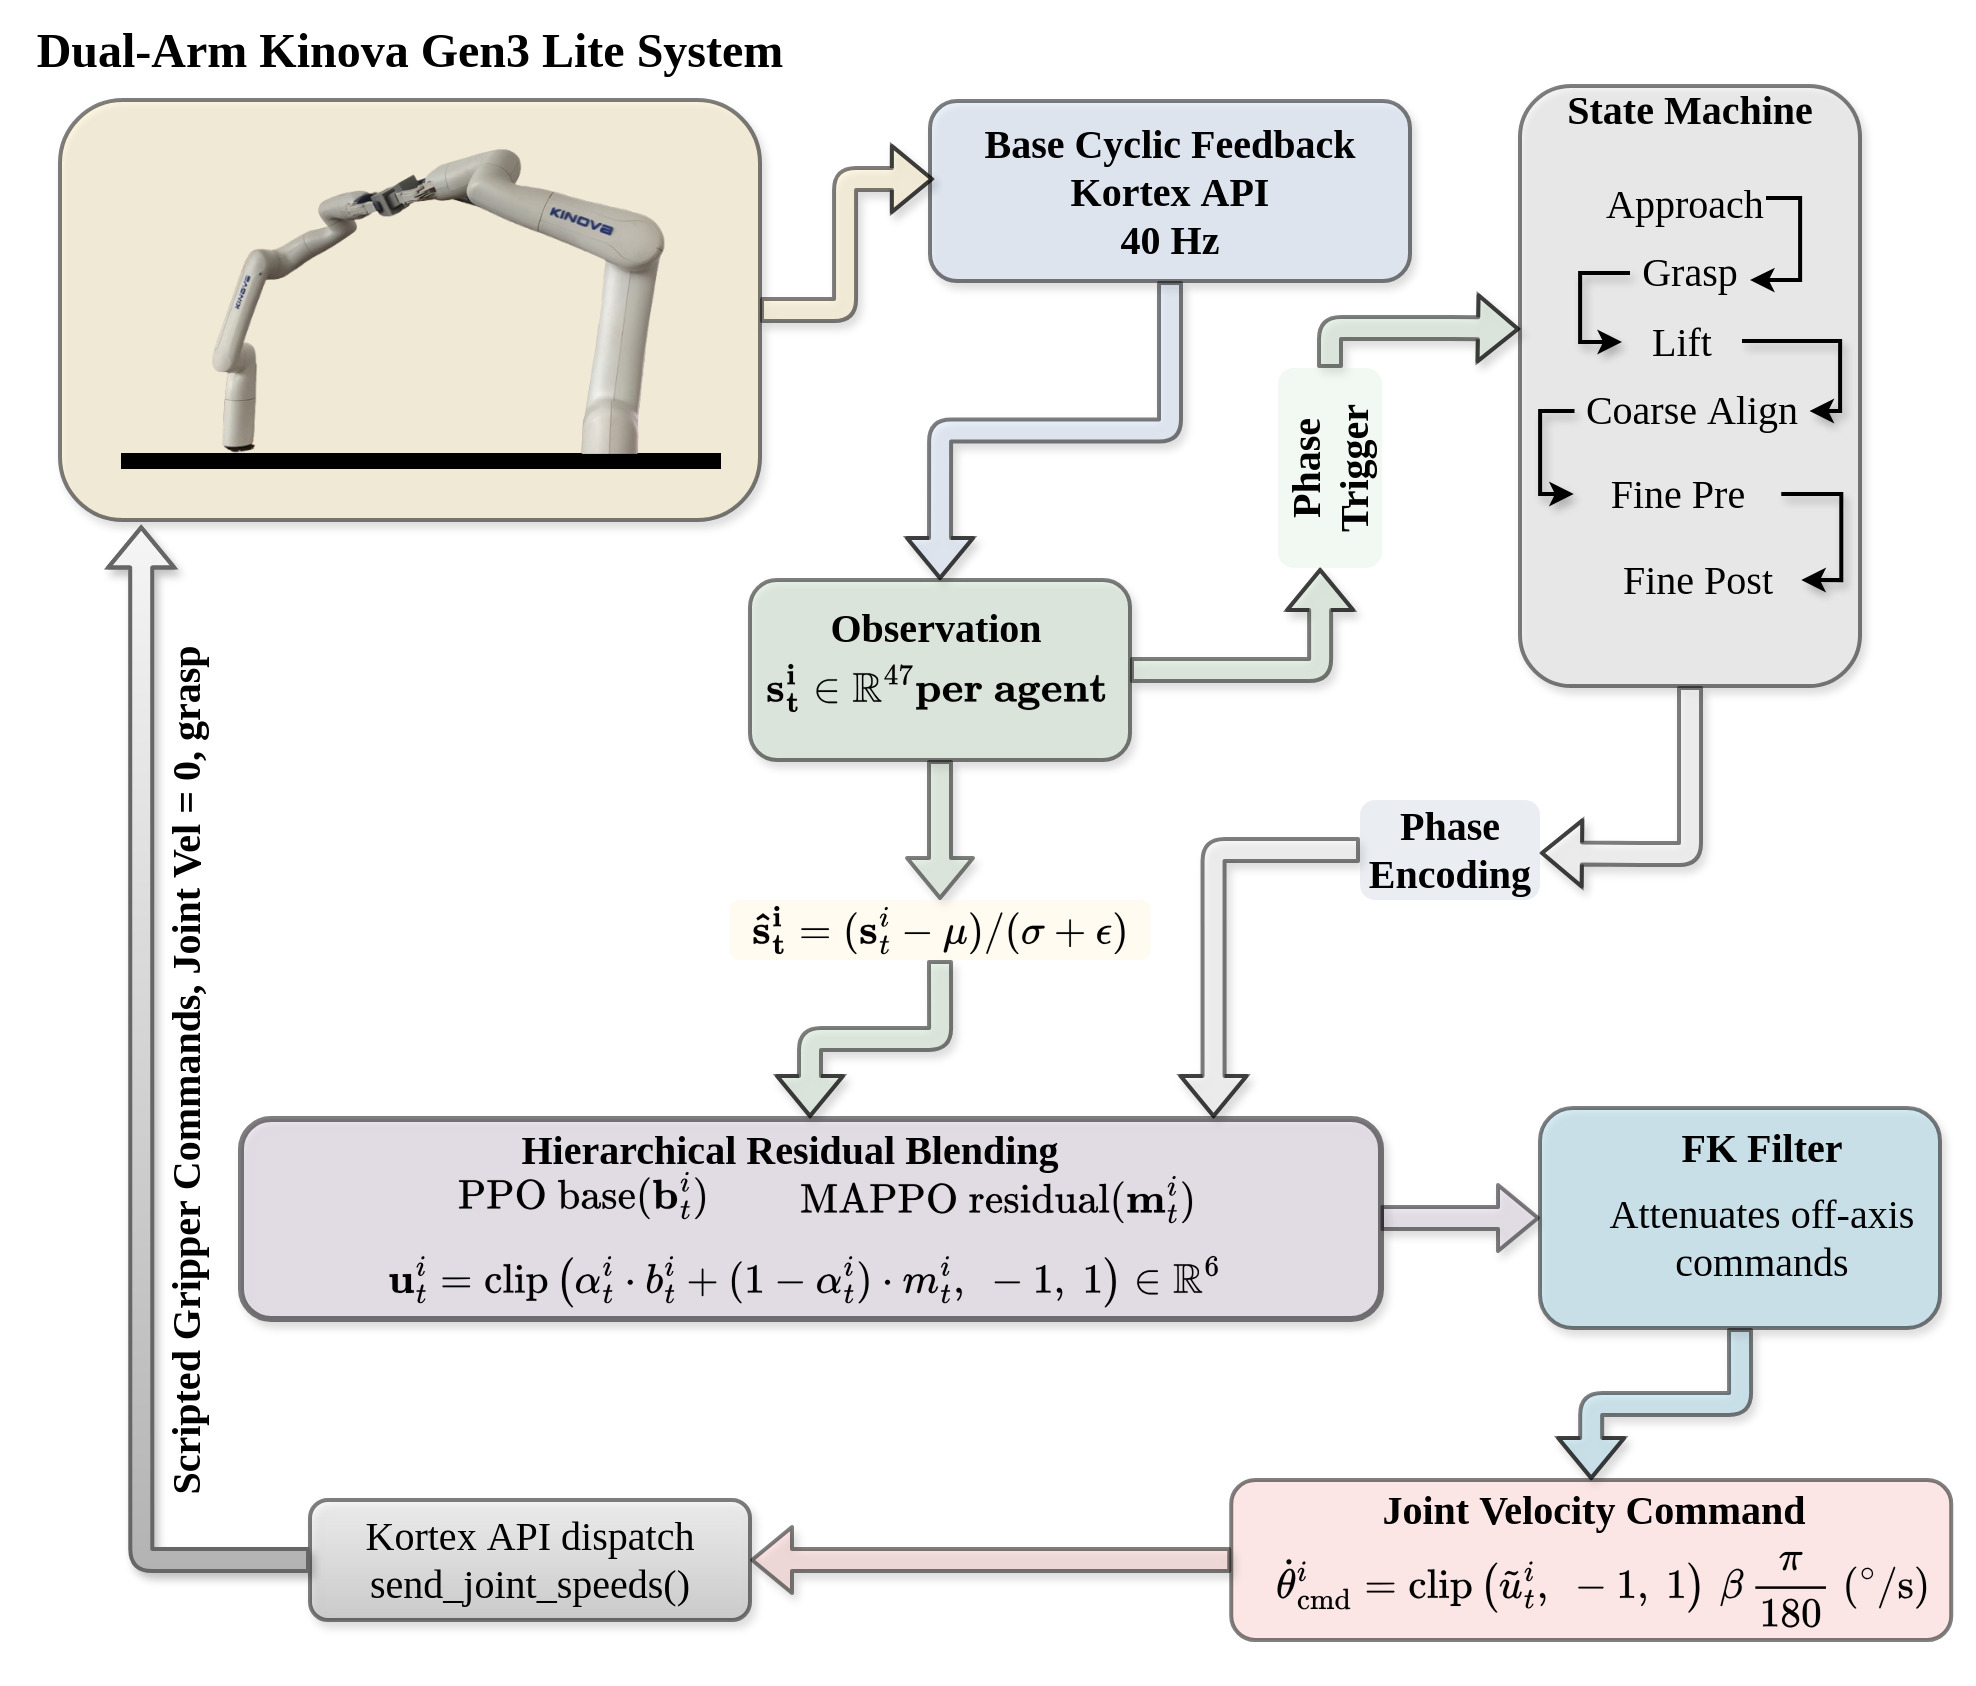
\includegraphics[width=0.7\linewidth]{Figures/TAI-Sim_2_real_deployment.jpg}
    \caption{Simulation to Real Hardware Deployment Architecture on Dual Kinova Gen3 Lite Manipulator System.}
    \label{fig:sim2real}
\end{figure}
Real-hardware deployment is governed by a state-machine controller implemented via the Kinova Kortex API, spanning active phases from initial approach to fine post-alignment. Phase transitions are triggered by the simultaneous satisfaction of positional and orientational error thresholds for both manipulators. The grasping phase is the sole exception to the policy-driven execution, during this interval, a discrete gripper command is issued. All remaining joint motion across the active phases is driven entirely by the hierarchical coordination blending policy.

The frozen PPO base policy $\pi_{\theta_{\text{ppo}}}$ is queried independently per arm to produce $\mathbf{b}_t^i$, the MAPPO actor $\pi_\theta$ produces the coordination policy $\mathbf{m}_t^i$ and blending increment $\mathbf{\Delta\alpha}_{t}^{i}$, and the final blended command $\tilde{\mathbf{u}}_t^i$ is computed per Eq.~(\ref{combined_action_noise}). The blended action is then scaled and converted to hardware joint velocity commands dispatched via the Kortex API as in Eq.~(\ref{hard_ware_vel}):
\begin{equation}
\dot{\theta}_{\text{cmd}}^i =
\mathrm{clip}\left( \tilde{u}_t^i,\ -1,\ 1 \right)\cdot\frac{\pi}{180}
\; (\mathrm{^\circ/s})
\label{hard_ware_vel}
\end{equation}
The phase one-hot encoding $\mathbf{e}_{\text{phase}} = [1, 0]^\top$ is maintained throughout approach, lift, and coarse alignment, switching to $\mathbf{e}_{\text{phase}} = [0, 1]^\top$ exclusively during fine alignment phases, exactly mirroring the simulation phase encoding seen during training.

During simulation training, a RunningStandardScaler maintains online estimates of the mean $\mu \in \mathbb{R}^{47}$ and standard deviation $\sigma \in \mathbb{R}^{47}$ of each agent's local observation $s_t^i$ as shown in Eq.~(\ref{normalized_obs}). These statistics are frozen at the end of training and applied to every real-hardware observation prior to policy inference:
\begin{equation}
    \hat{s}^{i}_{t} = (s^{i}_{t} - \mu)/(\sigma + \epsilon)
    \label{normalized_obs}
\end{equation}
The simulation snap mechanism, which triggers when the two offset end-effectors come within 8~cm and 0.2~rad of each other is not transferred to hardware. Without force sensing at fingers or active collision avoidance, triggering a proximity-based snap at close range risks object-to-object or arm-to-arm collision under any misalignment. Instead, the state machine enforces alignment through three predefined spatial separation waypoints, coarse alignment at 0.4~m offset end-effector separation, fine pre-alignment at 0.17~m, and fine post-alignment at 0.1~m. Progression to the next way point occurs only after both arms simultaneously satisfy position and orientation error thresholds at the current separation distance. This staged spatial approach eliminates the need for a collision avoidance module entirely, a significant deployment simplification while preserving the alignment quality achieved through learned coordination. Further, during fine alignment phases, a forward kinematics consistency check attenuates velocity commands that deviate significantly from the desired approach axis, providing a complementary hardware safety layer without modifying the policy architecture.
\section{Experiments and Results}
\label{results_and_discussion}
All experiments were conducted using the simulation environment detailed in Sec.~\ref{simulation_setup}. Each method was evaluated over 10 independent trials, each trial comprising 4,096 individual episodes. The success rates across all environments are reported in Table~\ref{tab:sim_success}. Additionally, Fig.~\ref{fig:base_line_comparisons} illustrates the comparative performance of each method, specifically showing the accumulated mean reward over the course of training. Relative success (Rel.Succ) is defined as the conditional alignment success rate among environments that successfully completed the reach phase.
\begin{figure}
    \centering
    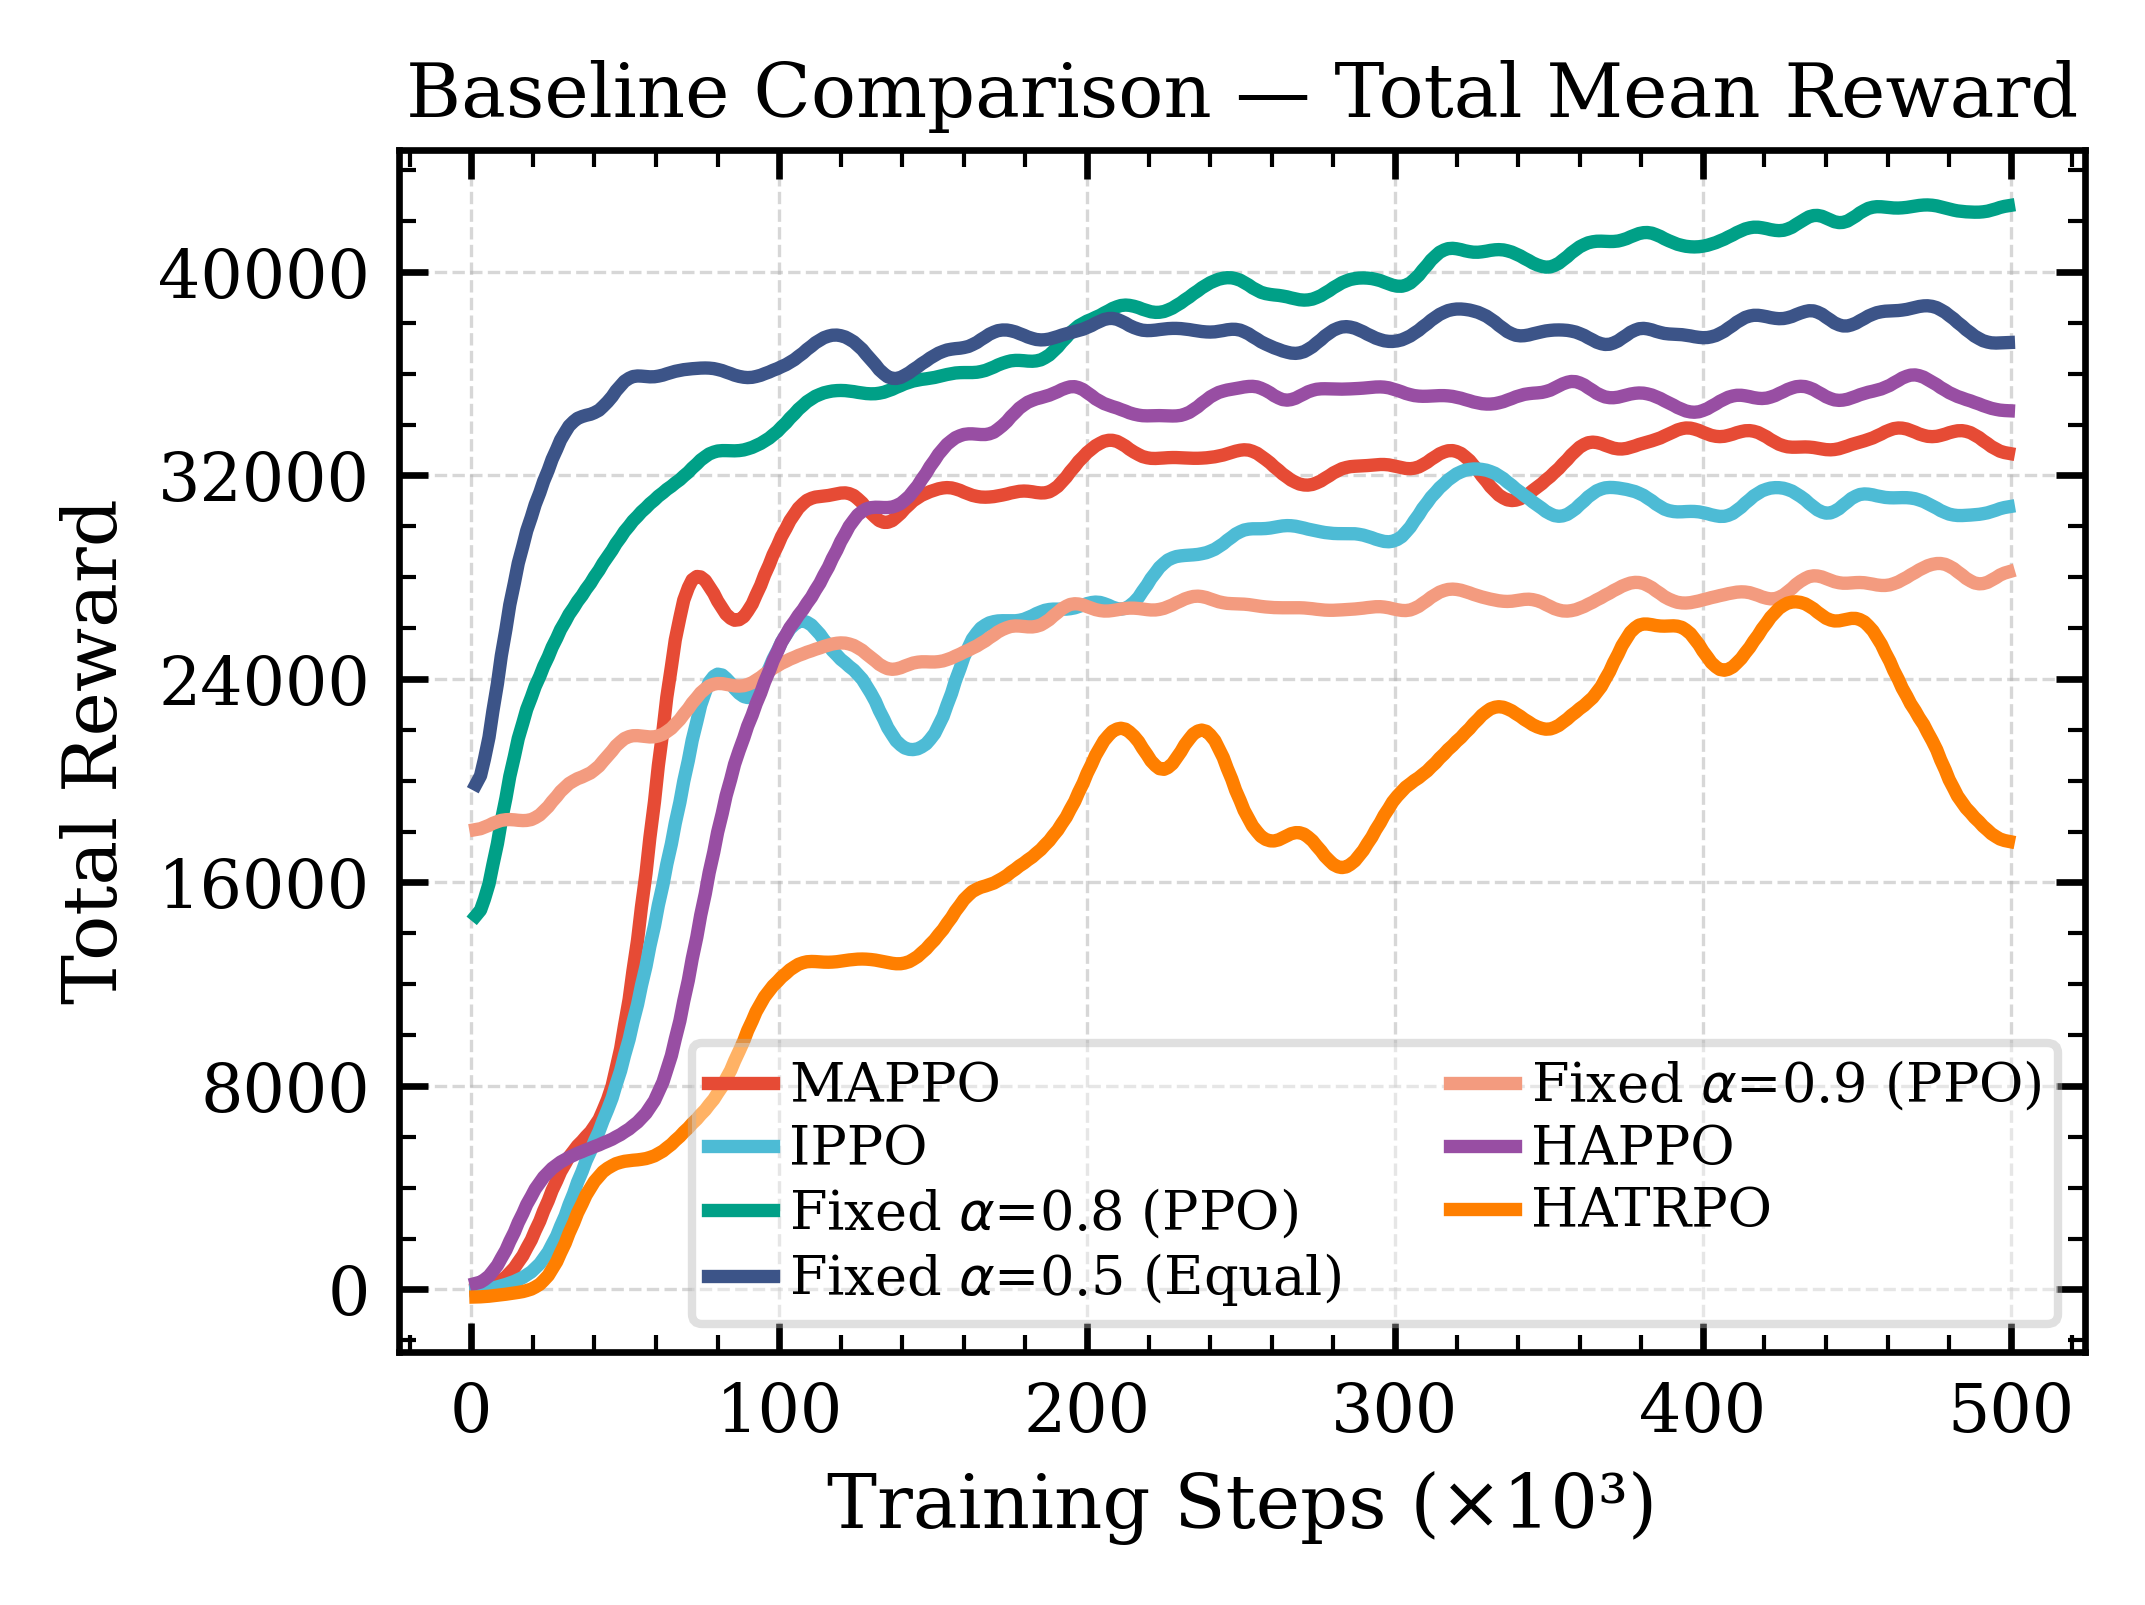
\includegraphics[width=\linewidth]{Figures/baseline_reward_plot_updated.png}
    \caption{Baseline Comparison: Total mean reward evolution of pure MARL algorithms and variants of MAPPO + PPO.}
    \label{fig:base_line_comparisons}
\end{figure}
\begin{table}[h]
\caption{Evaluation Results Over 10 Trials Across 4,096 Parallel Environments (Mean $\pm$ Std)}
\centering
\resizebox{\columnwidth}{!}{
\begin{tabular}{lccc}
\midrule 
\textbf{Method} & \textbf{Reach Succ(\%)} & \textbf{Align Succ(\%)} & \textbf{Rel.Succ(\%)} \\
\midrule \midrule
MAPPO \cite{MAPPO} & 71.6$\pm$0.5 & 8.3$\pm$0.3 & 11.6$\pm$0.5\\
HAPPO \cite{happo/htrpo} & \textbf{73.6$\pm$0.7} & \textbf{32.3$\pm$0.8} & 43.9$\pm$1.2 \\
IPPO \cite{IPPO} & 62.0$\pm$0.5& 25.0$\pm$0.3 & 40.3$\pm$0.6\\
HATRPO \cite{happo/htrpo} & 6.6$\pm$0.3 & 3.4$\pm$0.1 & 51.5$\pm$2.8 \\
PPO - MAPPO (0.5-0.5) & 41.1$\pm$0.8& 18.4$\pm$0.5 & 44.8$\pm$1.1\\
PPO - MAPPO (0.8-0.2) & 47.7$\pm$0.8& 17.6$\pm$0.8 & 36.9$\pm$1.3\\
PPO - MAPPO (0.9-0.1) & 1.76$\pm$0.2& 0.02$\pm$0.01 & 1.1$\pm$0.6\\
\midrule
\end{tabular}}
\vspace{2pt}
    \footnotesize{\textit{Note*:}} \textit{All pairwise differences between PPO+MAPPO (Adaptive) and baselines are statistically significant ($p < 0.001$, two-sample t-test).}
\label{tab:sim_success}
\end{table}

Table.~\ref{tab:sim_success} and Fig.~\ref{fig:base_line_comparisons} reveal critical performance trade-offs across all baseline configurations. Pure MAPPO achieves the highest reach success of (71.6\%), confirming that centralized training with a shared global critic enhances single-arm approach capability. However, its absolute alignment success collapses to 8.3\% with a conditional alignment rate of only 11.6\%. This exposes the fundamental sample complexity cost of learning low-level reachability and high-level cooperative alignment simultaneously from a single reward signal under joint policy optimization. In contrast, Pure IPPO achieves a higher absolute alignment success (25.0\%) and conditional alignment rate (40.3\%) despite an inferior reach rate (62.0\%). This inversion indicates that decentralized independent critics, while blind to the partner agent's state, encourage more conservative per-arm behaviors that reduce inter-agent interference during fine alignment convergence, at the direct cost of coordination quality as measured by the centralized reward signal. Although, HAPPO achieves the highest reaching success among MARL baselines (73.6\%), yet its alignment success (32.3\%) and conditional success rate (43.9\%) remain well below ALPHA. While HAPPO retains a centralized critic with global state access, its sequential actor update scheme, the mechanism providing its monotonic improvement guarantee updates each agent's policy in turn. Consequently, the other agent's advantage is computed against an shifted joint policy. In a bilateral alignment task requiring simultaneous inter-arm convergence, this sequential actor asymmetry directly disrupts the coordinated policy updates that require strict alignment demands. HATRPO collapses to near-total failure (6.6\% reach, 3.4\% alignment), with its reward curve uniquely regressing after 200k steps, a signature of hard KL-constrained updates proving incompatible with 12-DOF continuous joint velocity exploration, where the strict constraint repeatedly prevents escape from poor configurations. Its high Rel.Succ (51.5\%) is a statistical artifact of the near-zero reach denominator and carries no meaningful task interpretation.


Fixed-ratio blending reveals a critical and counterintuitive reward-success decoupling. Despite achieving the highest cumulative training rewards (Fig.~\ref{fig:base_line_comparisons}), fixed ratios of $\alpha^{i}_{t}=0.8 \text{ \& }0.5$ yield reach success of 47.7\% and 41.1\% respectively, below both pure methods with absolute alignment success of 17.6\% and 18.4\%, both well below Pure IPPO (25.0\%). Critically, their conditional alignment rates of 36.9\% ($\alpha^{i}_{t}=0.8$) and 44.8\% ($\alpha^{i}_{t}=0.5$) reveal that even among environments completing reach successfully, bilateral alignment coordination remains unreliable. Notably, $\alpha^{i}_{t}=0.8$ performs worse than Pure IPPO (40.3\%) on the conditional metric despite incorporating the frozen PPO prior, demonstrating that a rigidly dominant base policy actively suppresses the MAPPO coordination's capacity to enforce inter-arm coordination. While $\alpha^{i}_{t}=0.5$ marginally exceeds Pure IPPO on the conditional metric, its substantially lower reach success (41.1\% vs. 62.0\%) indicates the equal-weight blend interferes with single-arm approach convergence. The high cumulative rewards under fixed blending are explained by the PPO prior dominating action selection throughout the episode, producing smooth single-arm trajectories that accumulate dense per-step rewards without achieving bilateral task completion. The extreme case of $\alpha^{i}_{t}=0.9$ confirms this, reach success collapses to 1.76\%, conditional alignment to 1.1\%, and absolute alignment to effectively zero (0.02\%), yet the reward curve remains among the highest across all methods. This definitively demonstrates that cumulative reward is an unreliable proxy for cooperative task success in hierarchical multi-agent systems when the base policy contribution dominates the action space.

These findings jointly motivate the two core design choices of the proposed framework. The adaptive $\alpha^{i}_{t}$ mechanism avoids the fixed-ratio regimes by allowing each agent to dynamically regulate PPO prior reliance as a function of real-time coordination demand deferring to the base policy during independent reaching and suppressing it when bilateral convergence requires coordinated deviation. 

% Further, the CTDE via MAPPO provides the centralized critic with the global coordination signal necessary to bridge independent reaching and cooperative alignment, a structural capability absent in both Pure IPPO and all fixed-blend variants.
\begin{figure}
    \centering
    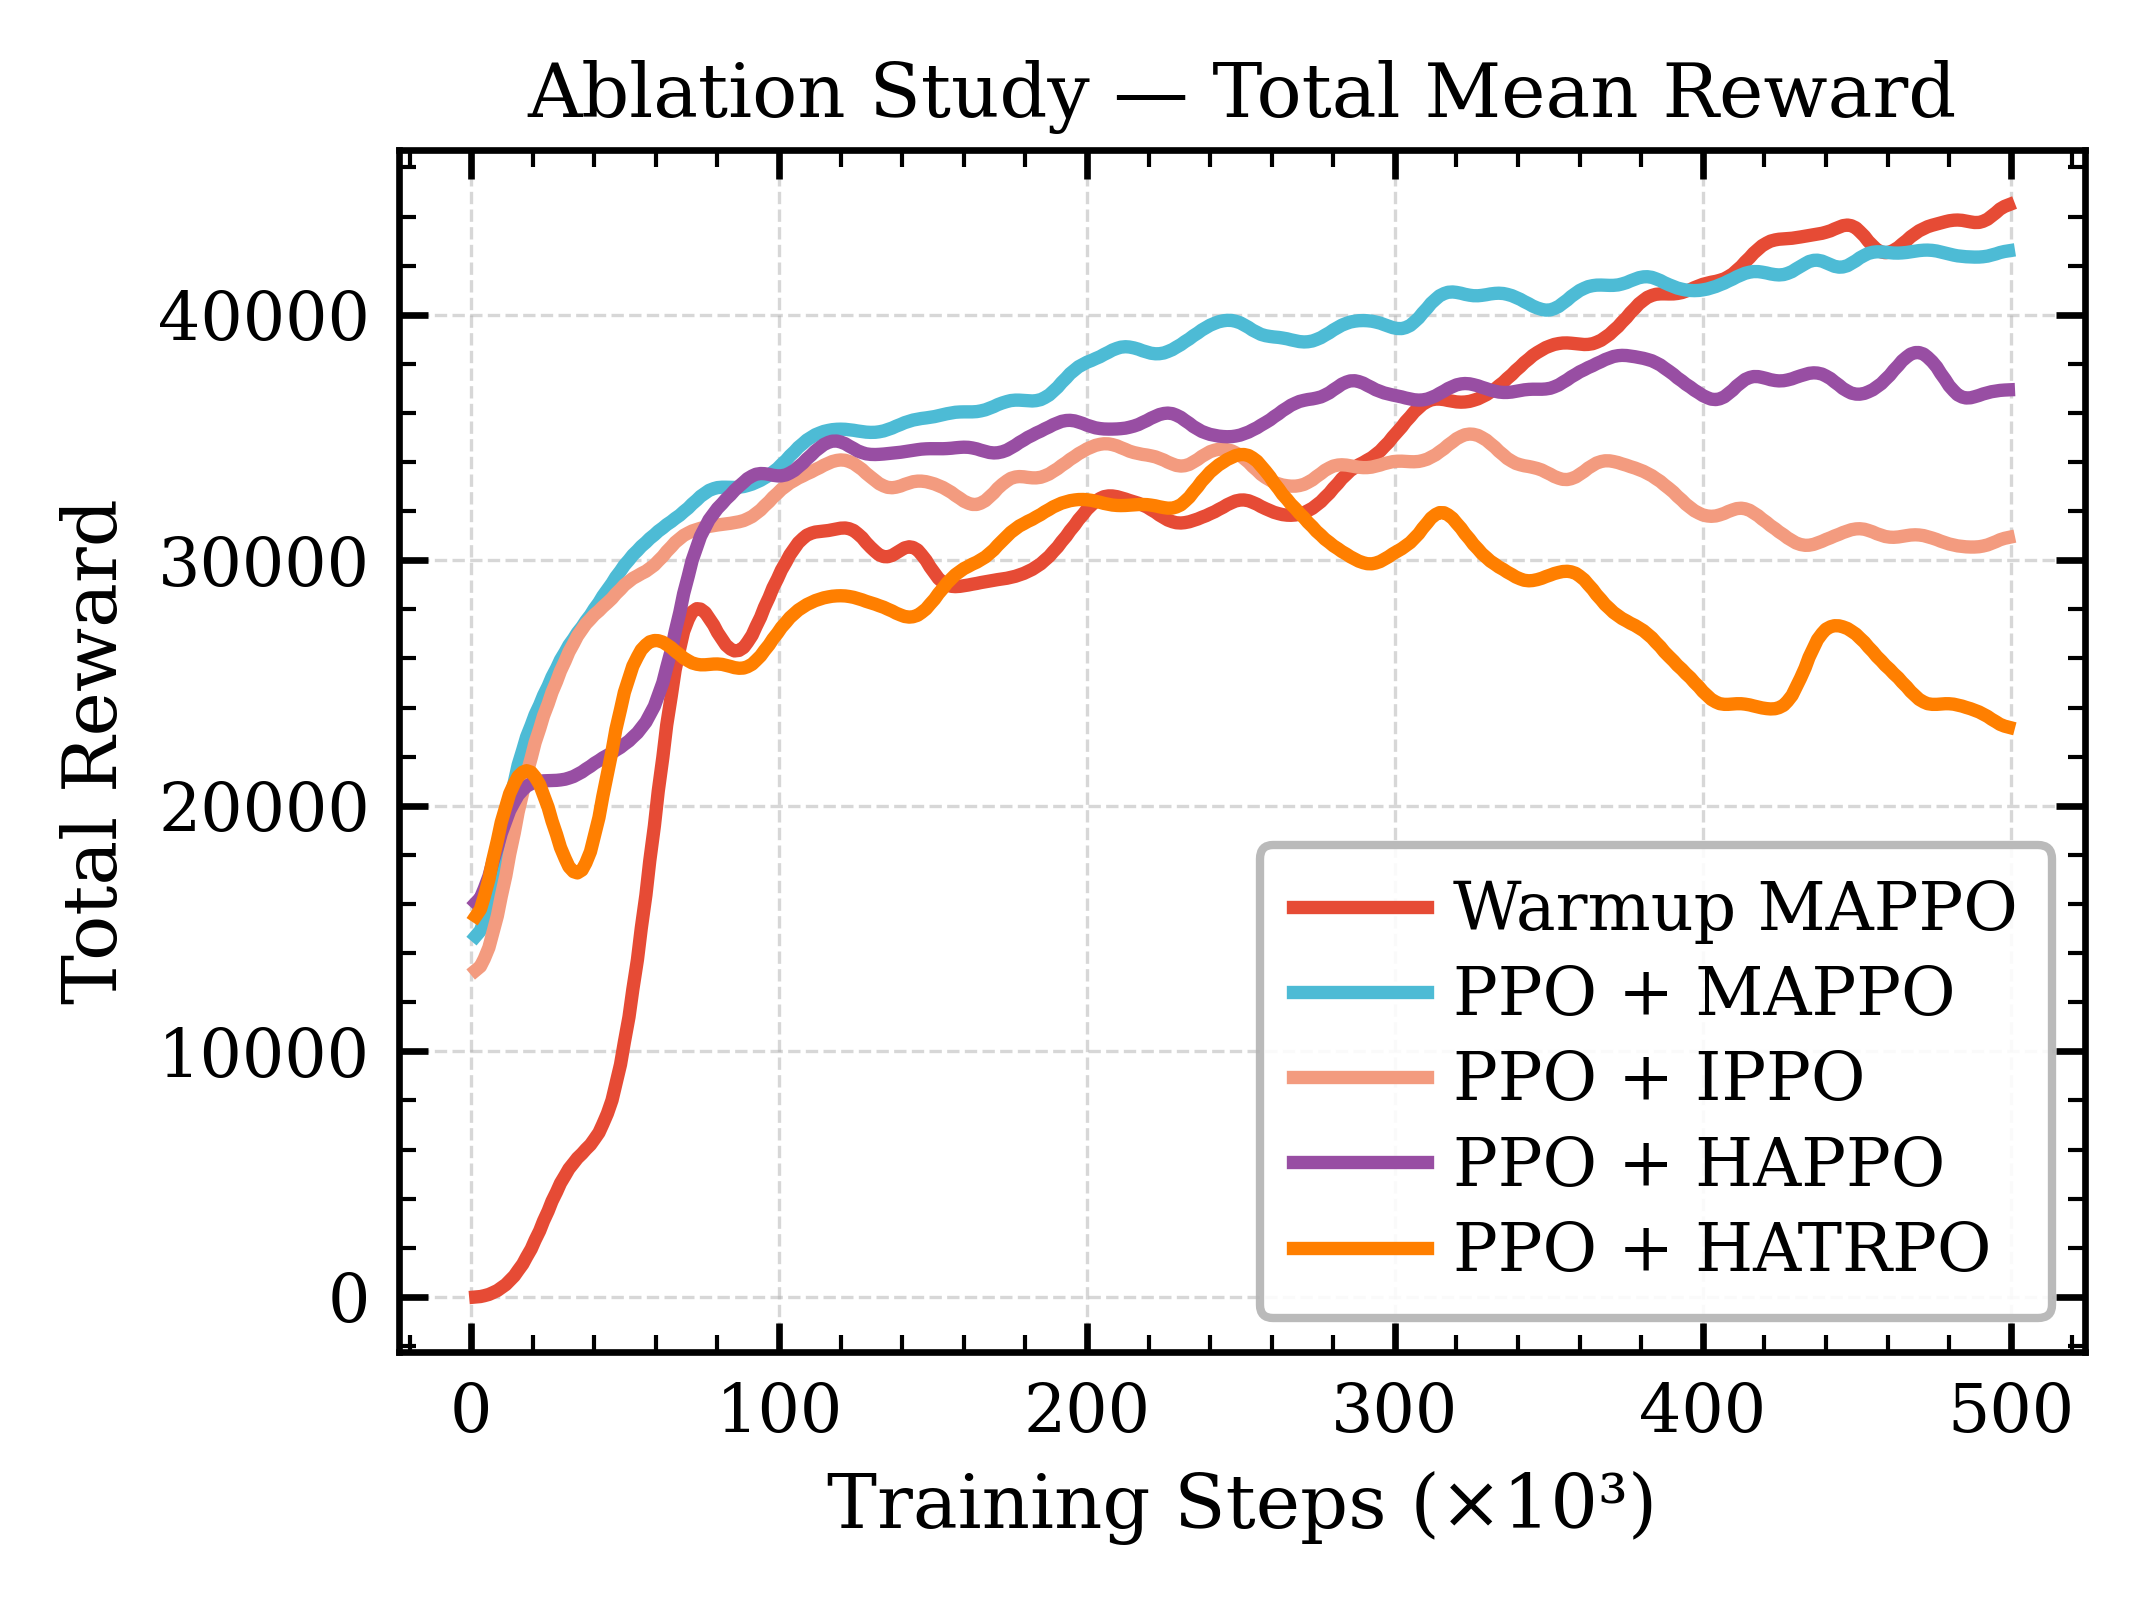
\includegraphics[width=\linewidth]{Figures/ablation_reward_plot_updated.png}
    \caption{Ablation Study: Total mean reward evolution of PPO + MAPPO(ALPHA) vs blending with existing MARL algorithms}
    \label{fig:ablation_study}
\end{figure}
\begin{table}[h]
\caption{Ablation Study Over 10 Trials Across 4,096 Parallel Environments (Mean $\pm$ Std)}
\centering
\resizebox{\columnwidth}{!}{
\begin{tabular}{lccc}
\midrule 
\textbf{Method} & \textbf{Reach Succ(\%)} & \textbf{Align Succ(\%)} & \textbf{Rel.Succ(\%)} \\
\midrule \midrule
Warmup MAPPO & 88.50$\pm$0.3& 85.80$\pm$0.2 & 96.94$\pm$0.3\\
\textbf{PPO - MAPPO (Adaptive)} & \textbf{96.50$\pm$0.3} & \textbf{95.0$\pm$0.4} & \textbf{98.45$\pm$0.4}\\
PPO - IPPO (Adaptive) & 67.50$\pm$0.7& 62.50$\pm$0.9 & 92.60$\pm$1.2\\
PPO - HAPPO (Adaptive) & 92$\pm$0.2 & 87$\pm$0.4 & 94.60$\pm$0.5\\
PPO - HATRPO (Adaptive) & 63.4$\pm$0.7 & 42.4$\pm$0.9 & 66.90$\pm$1.6\\
\midrule
\end{tabular}}
\vspace{2pt}
    \footnotesize{\textit{Note*:}} \textit{All pairwise differences are statistically significant ($p < 0.001$, two-sample t-test across 10 independent trials).}
\label{tab:ablation_metrics}
\end{table}

Table.~\ref{tab:ablation_metrics} and Fig.~\ref{fig:ablation_study} illustrate the individual contributions of adaptive blending, centralized training, and the warm-up curriculum. PPO+MAPPO (Adaptive, from t=0) achieves the highest performance across all metrics (96.5\% reach, 95.0\% alignment, and 98.45\% relative success), confirming that the combination of adaptive $\alpha^{i}_{t}$ and CTDE is the optimal configuration. PPO+IPPO (Adaptive), despite employing the same adaptive blending mechanism, yields substantially lower success in reaching (67.5\%), alignment (62.5\%), and relative success (92.59\%). This result directly demonstrates that the centralized critic is not redundant, without global state access during training, the decentralized coordination  policy cannot learn the precise bilateral coordination required for alignment convergence. The 32.5\% alignment gap and 5.86\% relative success gap between PPO+IPPO and PPO+MAPPO successfully isolates the contribution of CTDE independently of the blending mechanism. PPO+HAPPO, achieves 92\% reach and 87\% alignment with stable reward convergence, confirming that adaptive blending partially compensates for the absence of a centralised critic, yet the residual 8\% alignment gap to ALPHA persists, as the factored advantage estimates cannot fully substitute for global bilateral state during coordination learning. PPO+HATRPO, yields only 63.4\% reach and 42.4\% alignment, with reward regressing after 300k steps, demonstrating that the hard KL constraint instability is architecture-level and survives the addition of adaptive blending.

The Warmup MAPPO variant, which freezes $\alpha^{i}_{t}$ at zero for the first 150k timesteps before enabling adaptive blending, achieves 88.5\% reach, 85.8\% alignment, and 96.94\% relative success. While competent, it underperforms PPO+MAPPO (Adaptive) by approximately 9\% on reach and alignment, and 1.5\% on relative success. Its reward curve, shown in Fig.~\ref{fig:ablation_study}, exhibits a pronounced dip and delayed recovery around the 150k transition point, indicating that the abrupt introduction of blending after a pure MAPPO warmup disrupts the established policy. In contrast, PPO+MAPPO (Adaptive) enables blending from the initial timestep, allowing the policy to co-adapt the coordination policy and the blending gate jointly from the outset. 
\begin{figure}
    \centering
    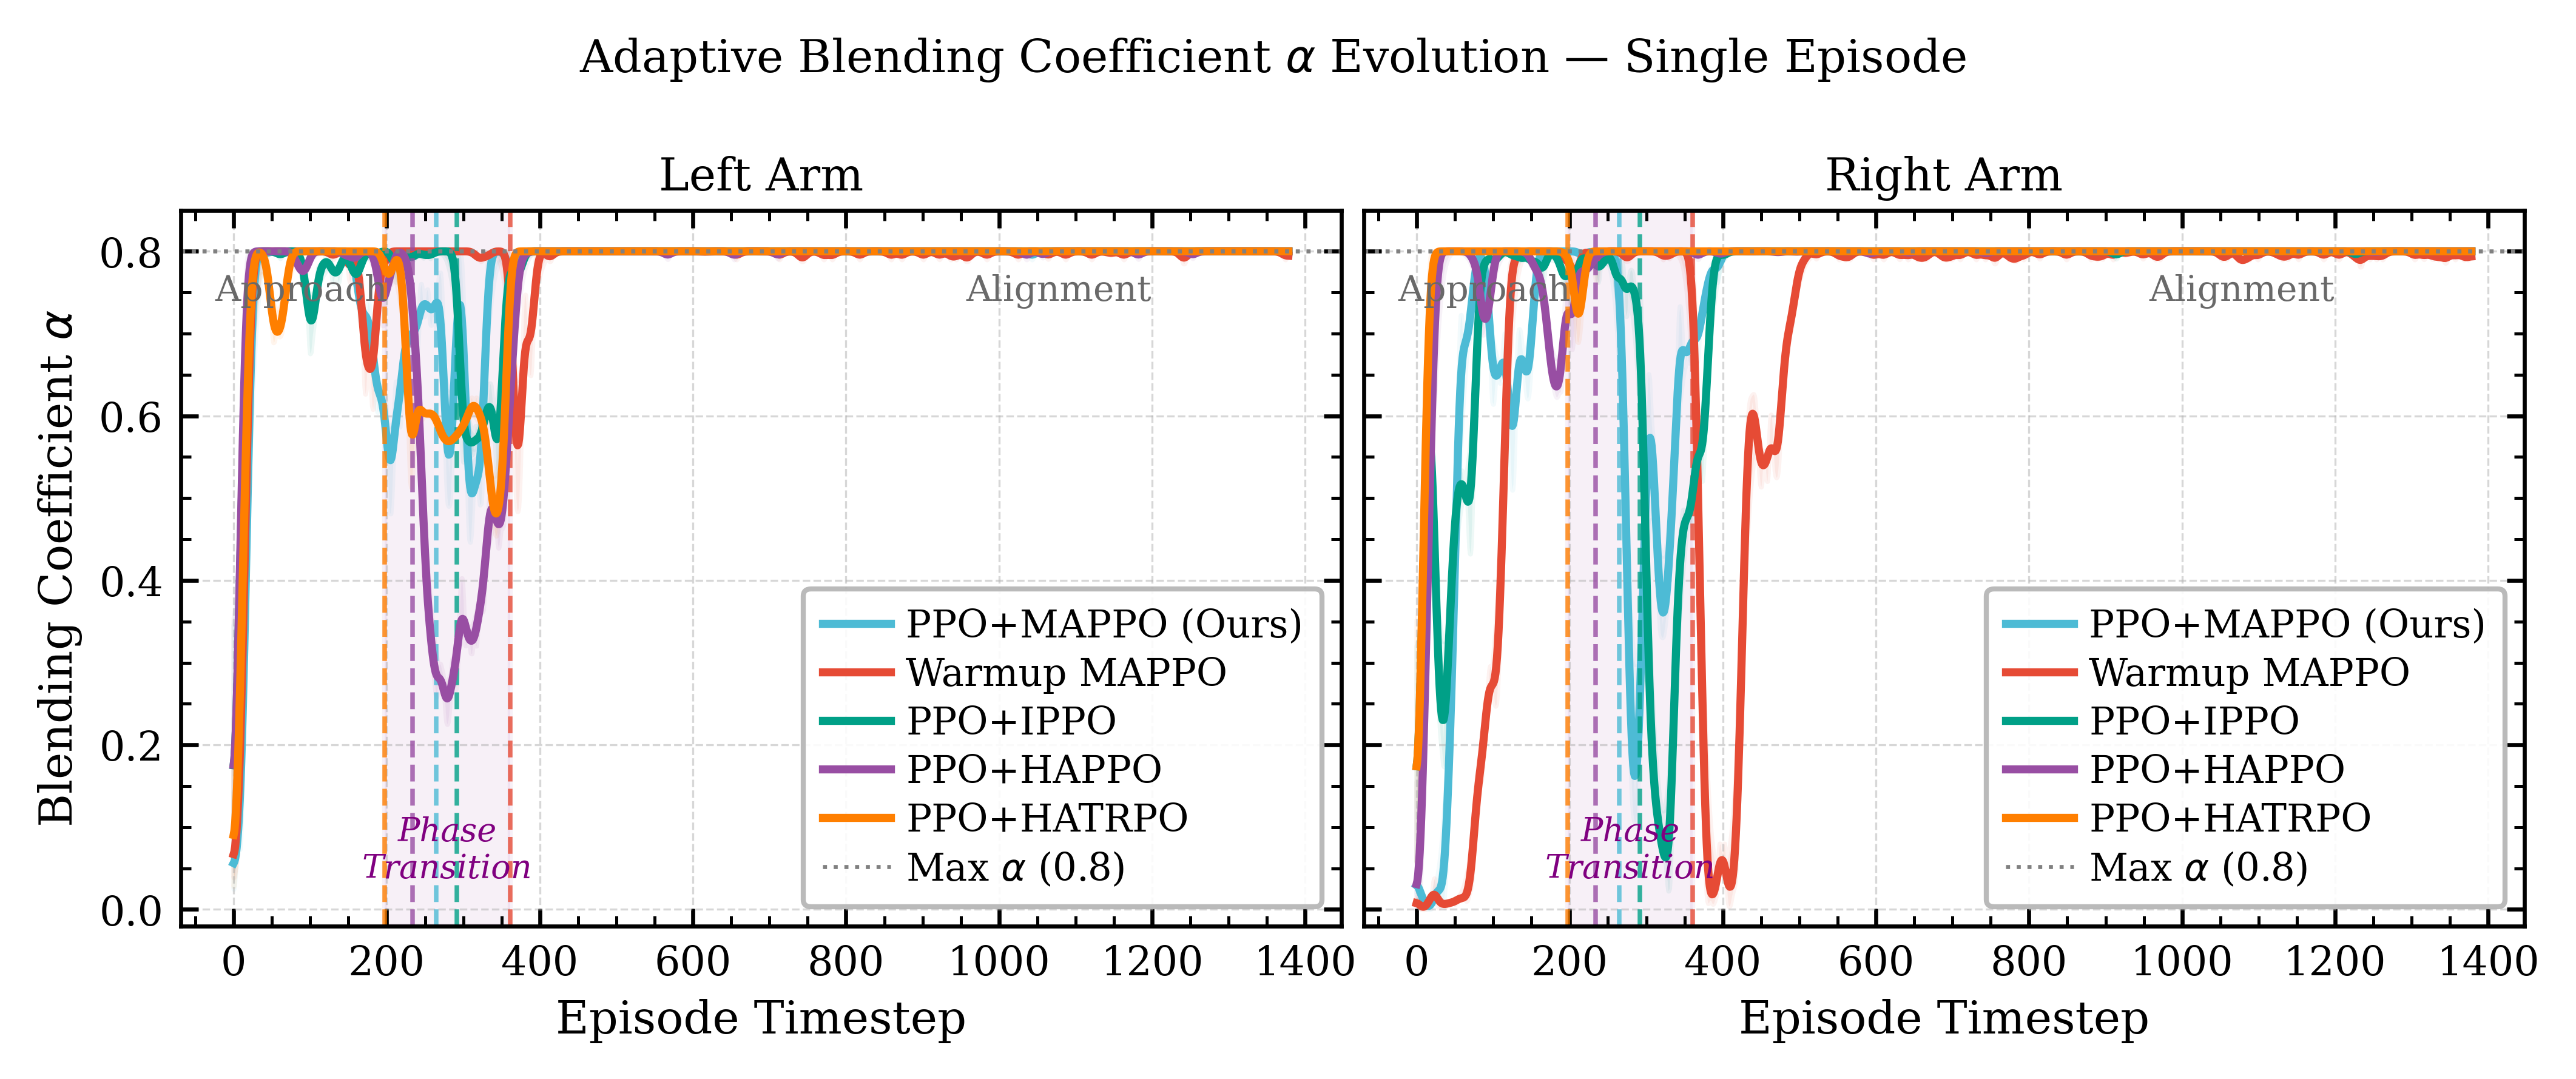
\includegraphics[width=\linewidth]{Figures/alpha_evolution.png}
    \caption{Comparison of methods' adaptive scale evolution over the episode.}
    \label{fig:alpha_evolution}
\end{figure}

Furthermore, Fig.~\ref{fig:alpha_evolution} shows $\mathbf{\alpha}^{i}_{t}$ evolution across a single episode for both arms. During approach, all methods rapidly saturate $\mathbf{\alpha}^{i}_{t}$ to 0.8, confirming the policy learns to maximally defer to the PPO prior for single-arm reaching. At the phase transition, all methods exhibit a pronounced $\mathbf{\alpha}^{i}_{t}$ reduction, the policy actively suppresses PPO reliance when cooperative alignment demands increase and independent reaching targets become counterproductive. This dip is the empirical justification for adaptive blending mechanism, any fixed $\mathbf{\alpha}^{i}_{t}$ would maintain inappropriate PPO dominance precisely when the task requires coordinated deviation. The asymmetric dip depth and recovery timing between the left and right arms across all methods reflects the structural asymmetry in their observation spaces. The left arm observes its own errors in its own frame while receiving the right arm's errors transformed into the left frame, and vice versa for the right arm. This produces distinct error magnitudes and gradient signals at the phase transition even under identical task conditions. This per-agent asymmetry is a direct consequence of the decentralized execution structure under CTDE, where each actor conditions on a locally-framed 47-D observation rather than a 92-D shared global representation. PPO+MAPPO (Ours) shows the shallowest and shortest dip on both arms, recovering fastest due to the centralized critic's global coordination signal. PPO+IPPO exhibits a deeper, oscillatory dip, decentralized critics cannot resolve the coupled bilateral alignment without global state access, and the asymmetry is more pronounced as each arm independently attempts to re-establish its gating strategy without awareness of the other's blending state. Warmup MAPPO shows a prolonged depression with delayed right-arm recovery, consistent with the reward instability in Fig.~\ref{fig:ablation_study}, where abrupt blending introduction after the 150K freeze disrupts co-adapted gating and coordination behaviors, with the right arm recovering more slowly due to its geometrically distinct workspace position relative to the alignment convergence point. PPO+HAPPO exhibits the deepest dip across both arms at phase transition, reflecting maximum uncertainty in prior reliance when bilateral coordination is demanded without global state access. PPO+HATRPO shows an erratic, non-monotonic trajectory at transition, partially recovering before dropping again consistent with the policy instability driven by hard KL constraint oscillations observed in Fig.~\ref{fig:ablation_study}.

Furthermore, real-time hardware experiments were conducted on two kinova gen3 lite manipulators, for collaborative dual-arm pick and alignment task of square and cylinder peg insertion in hole. 
\begin{figure}
    \centering
    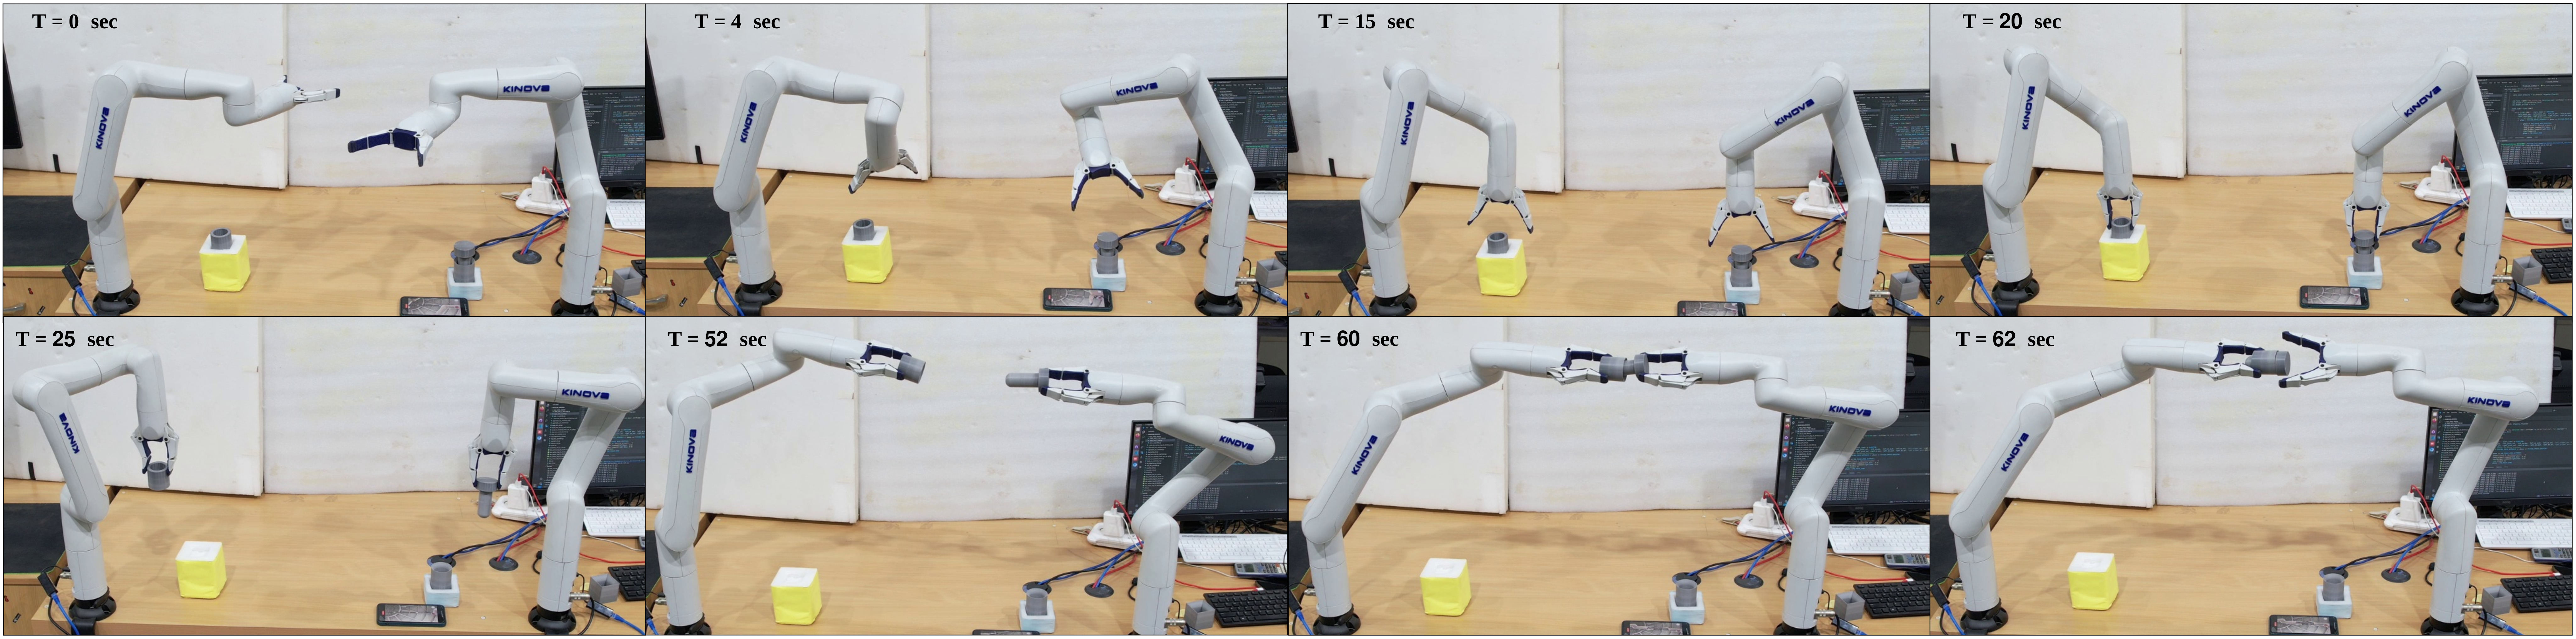
\includegraphics[width=\linewidth]{Figures/TAI-EXP_1.jpg}
    \caption{Experiment 1: Sequential execution of the dual-arm pick-and-pre-assembly alignment task of cylinder peg and hole on real Kinova Gen3 Lite hardware.}
    \label{fig:real_time_exp_1_sequential}
\end{figure}
\begin{figure}
    \centering
    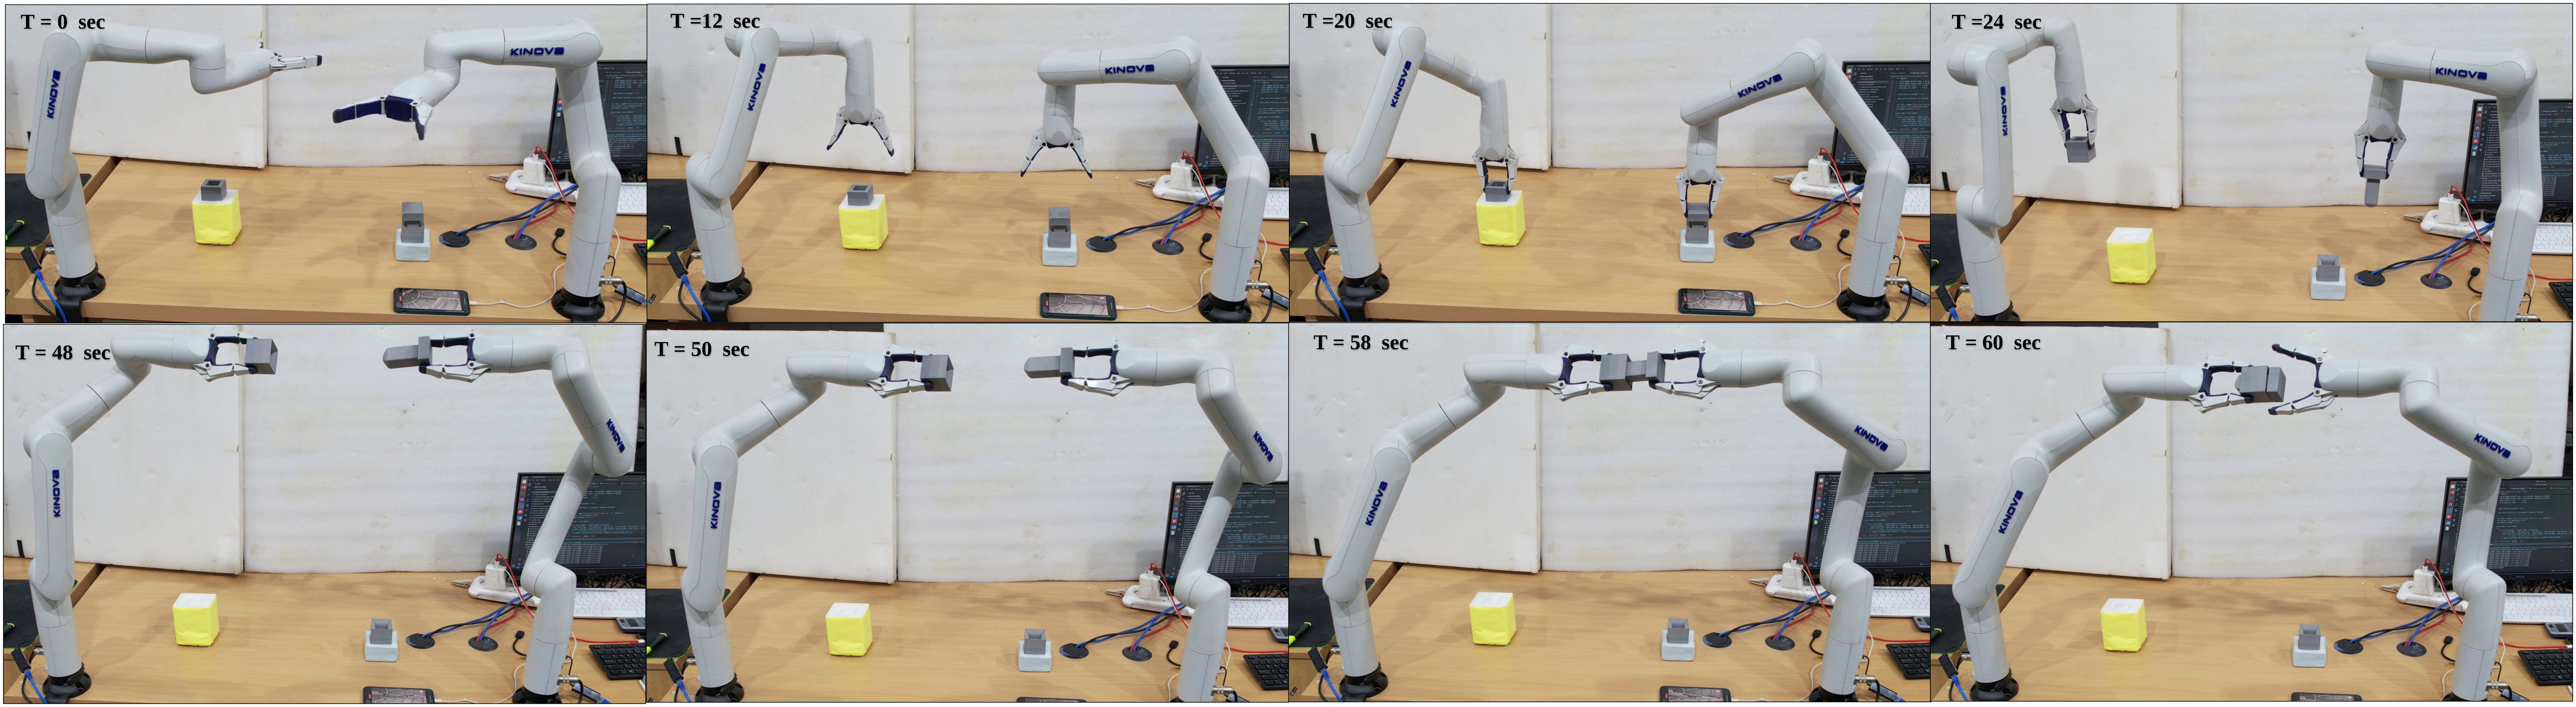
\includegraphics[width=\linewidth]{Figures/TAI-EXP-2.jpg}
    \caption{Experiment 2: Sequential execution of the dual-arm pick-and-pre-assembly alignment task of square peg and hole on real Kinova Gen3 Lite hardware.}
    \label{fig:real_time_exp_2_sequential}
\end{figure}
\begin{figure}
    \centering
    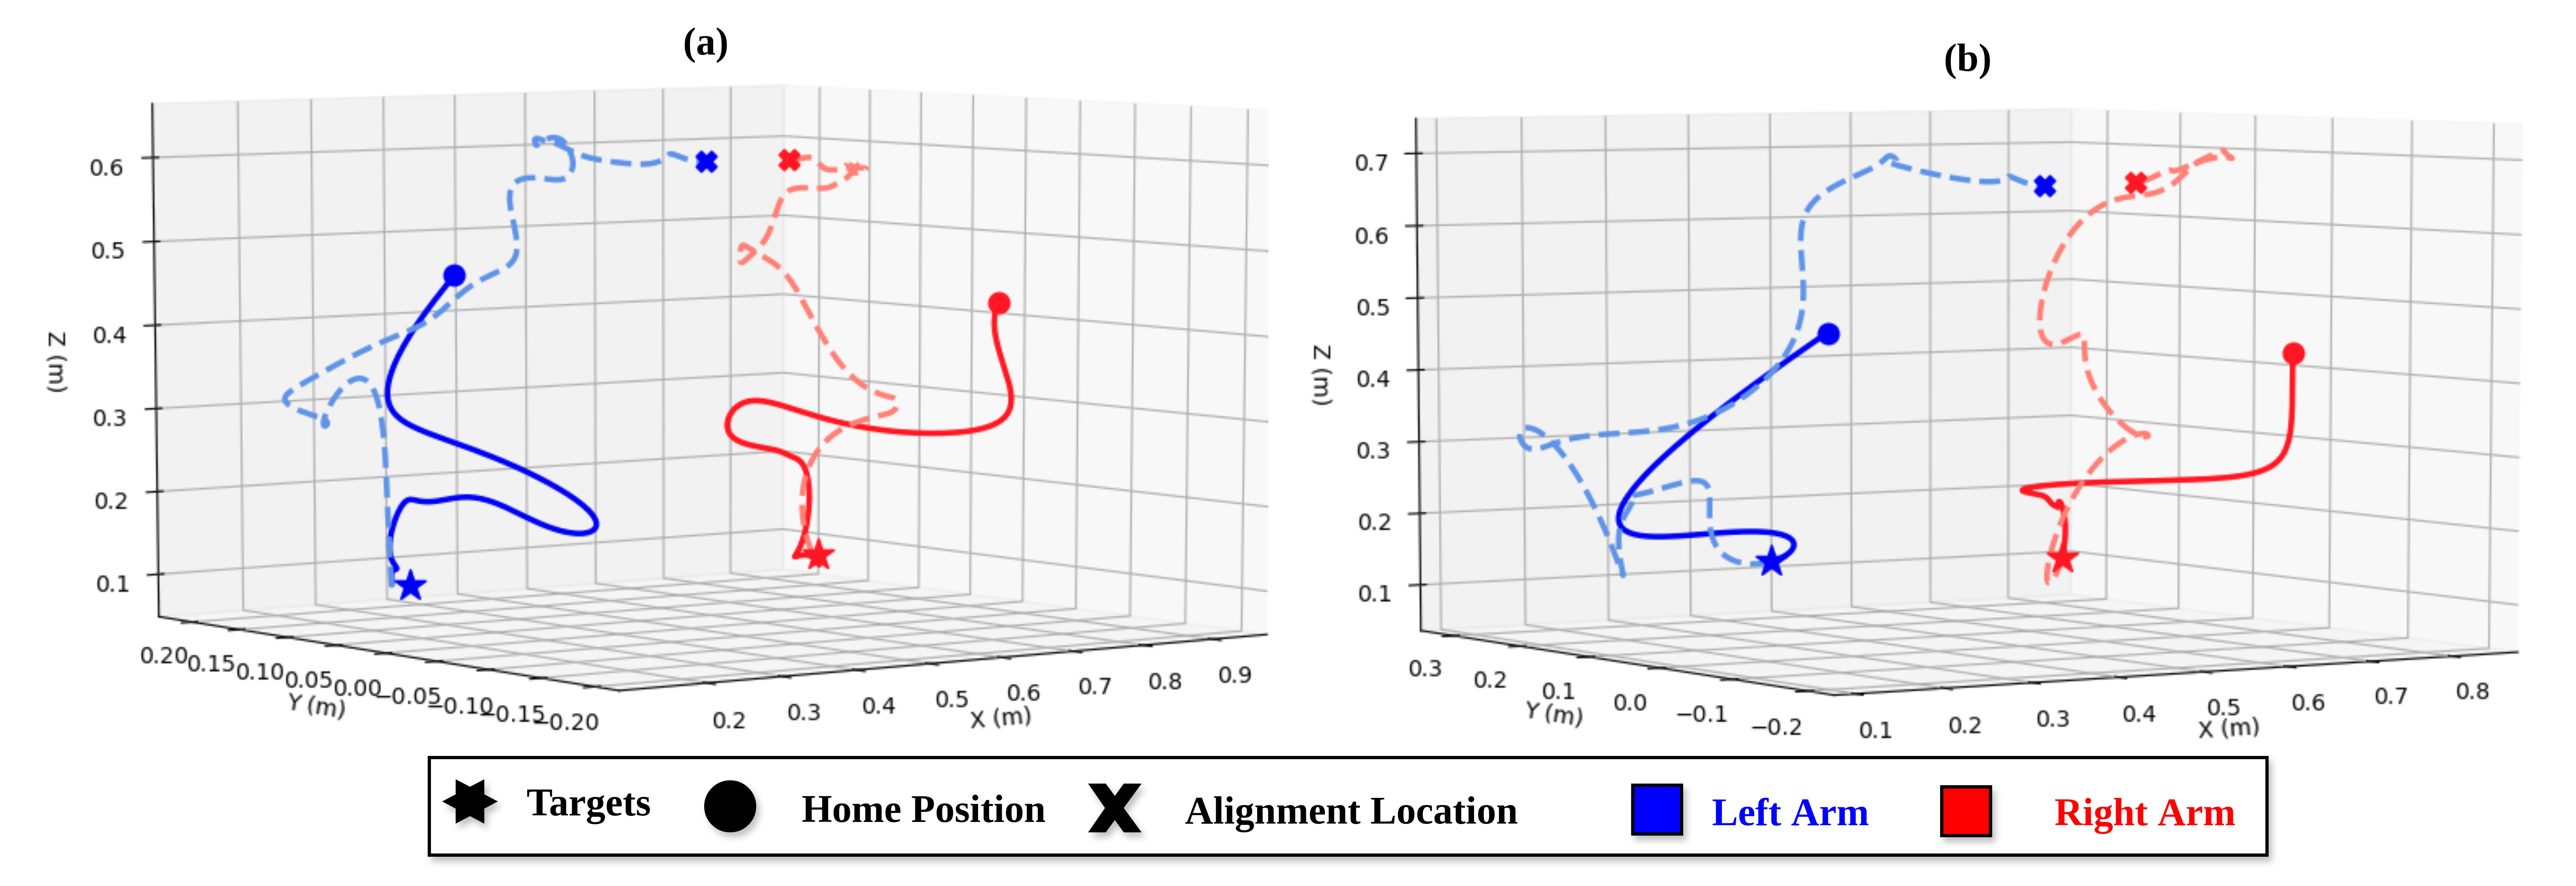
\includegraphics[width=\linewidth]{Figures/TAI-Page-3(1).jpg}
    \caption{End-effector trajectories of the dual-arm system during two real-hardware experiments. (a) Experiment 1 and (b) Experiment 2.}
    \label{fig:real_time_exp}
\end{figure}
The experimental setup consists of a cylindrical peg and a corresponding hole positioned within the reachable workspace of the dual-arm manipulator system, as illustrated in Fig.~\ref{fig:real_time_exp_1_sequential}. The arms begin from their respective home positions (T=0~s) and reach their targets by T=4~s. Following the simultaneous convergence of positional and orientational error thresholds in the X and Y directions, while maintaining a safe Z-offset from the targets at T=15~s, the arms descend vertically to grasp the objects at T=20~s. Subsequently, the manipulators move to a safe spatial clearance to prevent potential collisions at T=25~s, eventually reaching pre-docking positions at T=52~s. Finally, through collaborative axial alignment, the objects are successfully docked by T=60~s. A similar progression is observed for the second case in Fig.~\ref{fig:real_time_exp_2_sequential}. The corresponding end-effector trajectories for both cases are provided in Fig.~\ref{fig:real_time_exp}(a) and Fig.~\ref{fig:real_time_exp}(b), respectively.

\begin{table}[t]
\caption{Hardware Deployment Results Over 30 Trials with Varied Target Positions}
\label{hardware_result}
\centering
\footnotesize
\setlength{\tabcolsep}{4pt}
\renewcommand{\arraystretch}{1.2}
\begin{tabular}{l c c c}
\toprule
\textbf{Outcome} & \textbf{Reach} & \textbf{Align} & \textbf{Count} \\
\midrule
Successful execution            & $\checkmark$ & $\checkmark$ & 27 \\
Object slipped during insertion & $\checkmark$ & $\times$     & 1  \\
Gripper fault during grasping   & $\times$     & $\times$     & 2  \\
\midrule
\textbf{Success Rate} & \textbf{93.3\%} & \textbf{90.0\%}\textsuperscript{*} & \textbf{30} \\
\bottomrule
\end{tabular}

\vspace{2pt}
\footnotesize{\textit{Note*:}} \textit{Alignment success rate computed over all 30 trials. Relative alignment success over successful reach trials is 96.4\%. 95\% Wilson confidence intervals: Reach [78.7\%, 98.2\%], Alignment [74.4\%, 96.5\%].}
\end{table}
\section{Discussion}
\label{discussion}
The ALPHA framework hierarchically composes a frozen DIKPPO prior with a MAPPO coordination policy through adaptive gating scalar $\mathbf{\alpha}^{i}_{t}$, allowing the blending mechanism and coordination policy to co-evolve from timestep zero. The centralized 92-D critic provides the bilateral coordination signal that neither fixed-blend variants nor decentralized IPPO critics can replicate, while the reward-success decoupling at $\mathbf{\alpha}^{i}_{t}=0.9$ demonstrates that dense reward accumulation is an unreliable proxy for cooperative task completion in hierarchical MARL, a finding with implications beyond this architecture.
% The proposed ALPHA framework addresses cooperative dual-arm manipulation by hierarchically composing a frozen single-arm DIKPPO prior with a MAPPO coordination  policy through an adaptive gating scalar $\mathbf{\alpha}^{i}_{t}$. Instead of learning reachability and inter-arm coordination simultaneously from scratch, the coordination  policy operates exclusively in the blending action space, with $\mathbf{\alpha}^{i}_{t}$ co-evolving jointly with the coordination  from timestep zero. The centralized critic's 92-D global state provides the coordination signal necessary to bridge independent reaching and bilateral alignment, a capability that neither fixed-blend variants nor decentralized IPPO critics can replicate. The reward-success decoupling observed at $\mathbf{\alpha}^{i}_{t} = 0.9$, high cumulative reward, near-zero task success, further demonstrates that dense reward accumulation is an unreliable proxy for cooperative task completion in hierarchical MARL systems, a finding with implications beyond this specific architecture.

\noindent\textbf{Hardware Constraints:} The Kinova Gen3 Lite's non-spherical, force-sensor less gripper limits grasp verification to proximity thresholds; any in-hand slip propagates as an unobservable error into alignment. The min-operator bottleneck in (Eq.~\ref{pose_reward}) compensates for the restricted orientation space. Manipulators with integrated force sensing and spherical wrists would improve robustness with without structural changes to the blending or reward design, since force observations could be appended directly to $s^i_{t}$ and $S_t$.

% The Kinova Gen3 Lite's built-in two-fingered, non-spherical gripper without contact or force sensing imposes two compounding constraints. The gripping success is verified through proximity thresholds, any in-hand slip or object misalignment during lifting propagates as an unobservable error into the alignment phase. The non-spherical wrist geometry restricts the reachable orientation space, necessitating the min-operator bottleneck in the approach reward (Eq.~\ref{pose_reward}) to prevent the policy from optimizing position while accumulating orientation error. Manipulators with integrated force sensing at fingers and a spherical wrist would enable closed-loop grasp verification and compliant object handling during fine alignment. This directly improves the task robustness without requiring minimal architectural changes to the ALPHA policy, since force observations could be appended to the local observation $s^i_{t}$ and global critic state $S_t$. Further, hardware evaluation was conducted over 30 trials, while the observed success rates are consistent with simulation performance, wider confidence intervals inherent to this sample size suggest additional trials would further strengthen the deployment claim.

\noindent \textbf{Perception and Pose:} Object pose is assumed known a priori, an intentional scope boundary, not an architectural limitation. The ALPHA policy consumes only proprioceptive observations. A vision or pose estimation module would make the system perception-complete without modifying the learned policy or reward structure.
% The present framework assumes object pose is known a priori, with pick targets provided with in the reachable workspace. This is an intentional scope boundary rather than an architectural limitation. The ALPHA policy is fully agnostic to upstream perception, consuming only proprioceptive observations. Integration of a vision or pose estimation module of the state machine would make the system perception-complete without modifying the learned policy or reward structure, since object pose enters only as a target coordinate in the approach phase observation.

\noindent\textbf{Snap Mechanism and Sim-to-Real:} The simulation snap mechanism is excluded from hardware deployment, replaced by staged spatial waypoints at 0.4 m, 0.17 m, and 0.1 m separation, as detailed in Sec.~\ref{sim_2_real}. The 90\% hardware alignment success with snap fully replaced confirms that learned coordination is encoded in policy weights rather than reward structure. Although Isaac Lab provides contact force feedback, transferring contact observations to hardware would introduce observation distribution mismatch, further justifying the waypoint replacement.
% The simulation snap mechanism is excluded from hardware deployment. Triggering proximity-based snapping on real hardware without force sensing or active collision avoidance risks object-to-object and arm-to-arm collisions under any coordination  misalignment. The staged spatial waypoint strategy at 0.4 m, 0.17 m, and 0.1 m separation, as discussed in Sec.~\ref{sim_2_real}, enforces monotonic convergence without requiring a dedicated collision avoidance module. This represents a significant deployment modification. Although Nvidia Isaac Lab provides contact force feedback, transferring contact observations from simulation to hardware would introduce observation distribution mismatch. This discrepancy further justifies the waypoint replacement as the more transfer-stable design choice.

\noindent\textbf{Scalability:} The Dec-POMDP formulation is architecturally agnostic to agent count, extending to $N>2$ arms requires only expanding the global state dimensionality and adding agents to the MAPPO update, with no structural changes to the blending mechanism or reward design.
% The Dec-POMDP formulation with per-agent local observations and a shared global critic is architecturally agnostic to agent count. Extending to  $N>2$ arms requires only expanding the global state dimensionality and adding agents to the MAPPO update, with no structural changes to the blending mechanism or reward design, positioning the framework as a scalable foundation for multi-arm assembly beyond the dual-arm setting validated in this work.

\section{Conclusion}
\label{conclusion}
This work presented ALPHA, a cooperative dual-arm pre-assembly alignment framework composing a frozen DIKPPO prior with a MAPPO coordination policy through a learned adaptive gating scalar $\alpha^{i}_{t}$ output as a seventh action dimension. Joint training of coordination and gating from timestep zero under CTDE with a 92-D global critic achieves 96.5\% reach and 95.0\% alignment across 4,096 parallel simulation environments, significantly outperforming pure MAPPO (8.3\%), pure IPPO (25.0\%), HAPPO (32.3\%), HATRPO (3.4\%), all fixed-blend variants, and the warmup curriculum. Direct sim-to-real transfer on dual Kinova Gen3 Lite manipulators, with 200 Hz policy inference operating at 10x the 20 Hz hardware control loop on a CPU-only platform, demonstrates successful square and cylindrical peg-in-hole alignment. Future work will integrate force sensing for compliant contact handling, visual perception for object pose estimation, and extension to $N>2$ arm configurations.

% This work presented an Adaptive Learned Policy Hierarchical blending Architecture (ALPHA) framework for cooperative dual-arm pick-and-pre-assembly alignment. A frozen single-arm DIKPPO prior provides stable joint velocity priors, while a MAPPO coordination  policy learns inter-arm coordination through an adaptive gating scalar $\alpha^{i}_{t}$ output as a seventh action dimension. The simultaneous training of the coordination  and gating policies from timestep zero, under the CTDE paradigm with a 92-D global state critic, achieves 96.5\% reach and 95.0\% alignment success across 4,096 parallel simulation environments. This performance significantly outperforms pure MAPPO (8.3\% alignment), pure IPPO (25.0\%), all fixed-blend variants, and the 150k-MAPPO warmup curriculum. The adaptive $\alpha^{i}_{t}$ mechanism effectively eliminates the need for manual blend ratio tuning while enabling the policy to autonomously modulate prior reliance as a function of real-time coordination demand. Direct sim-to-real transfer onto dual Kinova Gen3 Lite manipulators via the Kortex API at 20 Hz demonstrates successful square and cylindrical peg-in-hole alignment at a 200 Hz policy inference rate on a CPU-only Intel NUC9 platform. Future work will focus on the integration of force sensing for compliant contact handling and the inclusion of visual perception for object pose estimation. Furthermore, extending this framework to $N > 2$ arm configurations for more complex assembly operations will further advance learning-based intelligent manipulation in industrial automation.

\bibliographystyle{ieeetr}
\bibliography{ref}
\end{document}


